\documentclass[lettersize,journal]{IEEEtran}
\usepackage{amsmath,amsfonts}
\renewcommand{\ttdefault}{cmtt}
\usepackage{array}
\usepackage[caption=false,font=normalsize,labelfont=sf,textfont=sf]{subfig}
\usepackage{textcomp}
\usepackage{url}
\usepackage{verbatim}
\usepackage{graphicx}
\usepackage{cite}
\usepackage{amssymb}
\usepackage{booktabs}
\usepackage[table]{xcolor}
\usepackage{microtype}
\microtypesetup{expansion=false}
\usepackage{makecell}
\usepackage{multirow}
\graphicspath{{./}}
\hyphenation{op-tical net-works semi-conduc-tor IEEE-Xplore}
% updated with editorial comments 8/9/2021

\usepackage{iftex}
\ifXeTeX
  \DeclareFontShape{TU}{ptm}{b}{n}{<->ssub * lmr/bx/n}{}
  \DeclareFontShape{TU}{ptm}{bx}{n}{<->ssub * lmr/bx/n}{}
  \DeclareFontShape{TU}{ptm}{b}{it}{<->ssub * lmr/bx/it}{}
  \DeclareFontShape{TU}{ptm}{bx}{it}{<->ssub * lmr/bx/it}{}
  \DeclareFontShape{TU}{ptm}{b}{sc}{<->ssub * lmr/bx/n}{}
  \DeclareFontShape{TU}{ptm}{bx}{sc}{<->ssub * lmr/bx/n}{}
  \DeclareFontShape{TU}{ptm}{m}{scit}{<->ssub * lmr/m/it}{}
\else
  \ifLuaTeX
    \DeclareFontShape{TU}{ptm}{b}{n}{<->ssub * lmr/bx/n}{}
    \DeclareFontShape{TU}{ptm}{bx}{n}{<->ssub * lmr/bx/n}{}
    \DeclareFontShape{TU}{ptm}{b}{it}{<->ssub * lmr/bx/it}{}
    \DeclareFontShape{TU}{ptm}{bx}{it}{<->ssub * lmr/bx/it}{}
    \DeclareFontShape{TU}{ptm}{b}{sc}{<->ssub * lmr/bx/sc}{}
    \DeclareFontShape{TU}{ptm}{bx}{sc}{<->ssub * lmr/bx/sc}{}
    \DeclareFontShape{TU}{ptm}{m}{scit}{<->ssub * lmr/m/it}{}
  \fi
\fi

\begin{document}

\title{MV-RaCL: Multi-View Role-Aware Contrastive Learning for Composition-Sensitive Semantic Matching}

\author{Minfeng Lu, Qifei Zhang, Hanlin Qin, Huilai Zou
\thanks{This work was supported by the General Scientific Research Project of Zhejiang Provincial Department of Education under Grant Y202456413. \textit{(Corresponding author: Huilai Zou.)}}
\thanks{Minfeng Lu, Hanlin Qin, and Huilai Zou are with the School of Artificial Intelligence, Zhejiang Polytechnic University of Mechanical and Electrical Engineering, Hangzhou 310053, China (e-mail: luminfeng@zime.edu.cn; qinhanlin@zime.edu.cn; zouhuilai@zime.edu.cn).}
\thanks{Qifei Zhang is with the School of Software Technology, Zhejiang University, Ningbo 315048, China (e-mail: cstzhangqf@zju.edu.cn).}}

% The paper headers
\markboth{IEEE Transactions on Emerging Topics in Computational Intelligence}%
{Lu \MakeLowercase{\textit{et al.}}: MV-RaCL: Multi-View Role-Aware Contrastive Learning}

%\IEEEpubid{0000--0000/00\$00.00~\copyright~2024 IEEE}
% Remember, if you use this you must call \IEEEpubidadjcol in the second
% column for its text to clear the IEEEpubid mark.

\maketitle

\begin{abstract}
This paper presents MV-RaCL, a multi-view role-aware contrastive learning framework that significantly improves composition-sensitive semantic matching. Existing prompt-based contrastive encoders adopt a \emph{role-agnostic} strategy---sharing one encoder path and contrastive temperature across views---which blurs representation boundaries and entangles gradient signals under compositional confounders (e.g., negation, subject--object swapping). We address this by introducing a View-Role Inductive Bias (VRIB) that explicitly differentiates anchor, positive, and hard-negative training views. Specifically, we construct three-view prompts at the template level, apply view-dependent asymmetric embedding dropout at the encoding level, and optimize a dual-temperature hard-negative InfoNCE objective that softly redistributes gradient mass. We evaluate MV-RaCL under a self-contained unsupervised BERT-base setting. Without external teachers or reference corpora, our model improves SICK-R Spearman from $71.41$ to $74.65$ ($+3.24$) over the CoT-BERT baseline, while keeping general STS-B performance stable. We also show---through controlled ablations, representation-space geometry, and per-phenomenon spot-checks---that this role-aware mechanism induces a \emph{selective compositional sharpening}, yielding more reliable alignment and separation boundaries for compositional semantics.
\end{abstract}

\begin{IEEEkeywords}
Sentence representation, Semantic matching, Compositional semantics, Contrastive learning, Prompt-based learning, View-Role Inductive Bias, SICK-R, Selective compositional sharpening.
\end{IEEEkeywords}

\section{Introduction}
\label{sec:intro}


\IEEEPARstart{S}{entence} representation learning aims to map natural language into a numerical vector space that captures semantic proximity, serving as a cornerstone for diverse downstream applications such as semantic textual similarity (STS), information retrieval, and paraphrase detection~\cite{sts3kcl}.

Since the introduction of SimCSE~\cite{simcse}, substantial strides have been made in unsupervised sentence embedding using discriminative pre-trained language models (PLMs) like BERT~\cite{bert}. Methods such as PromptBERT~\cite{promptbert} and CoT-BERT~\cite{cotbert} further refine representation quality by embedding inputs into structured natural-language prompts. However, in practical matching scenarios, the most critical risk is not distinguishing lexically dissimilar texts, but identifying \emph{compositional confounders}---sentence pairs that share the bulk of their lexical content yet express markedly different propositions due to negation, subject--object swapping, or predicate substitution. For encoders relying on cosine similarity, such high-overlap pairs frequently induce inflated scores and systematic misjudgments, a challenge specifically targeted by the SICK-Relatedness (SICK-R)~\cite{sick} benchmark.

Despite their success, existing prompt-based contrastive strategies typically encode anchor, positive, and hard-negative views in a highly \emph{role-agnostic} manner. They share the same encoder path, receive identical perturbation strength, and are optimized under a single contrastive temperature. While effective for basic semantic alignment, this structural property fails under compositional confounders: at the representation level, positives and hard negatives become geometrically too close, blurring discriminative boundaries; at the optimization level, a single temperature cannot separately calibrate the gradient demands of positive alignment versus hard-negative separation, entangling the objective signals. Although recent ranking-augmented methods~\cite{rankcse,rankencoder} leverage external reference corpora or supervised NLI signals~\cite{raoe} to reshape embedding geometry, their reliance on auxiliary resources drastically increases system complexity and computational cost, limiting their applicability in resource-constrained unsupervised settings.

This structural limitation motivates us to rethink the encoding and optimization mechanism of prompt-based contrastive learning. We propose MV-RaCL, a novel framework designed to construct more reliable alignment and separation boundaries for compositional semantics. Central to our approach is a unified View-Role Inductive Bias (VRIB) that applies role-differentiated treatments to the anchor, positive, and hard-negative views. Specifically, we explicitly delineate view roles via three-view prompt construction at the template level, inject view-dependent asymmetric dropout at the encoding level without introducing extra parameters, and utilize a dual-temperature hard-negative InfoNCE objective at the loss level. MV-RaCL strictly follows the unsupervised BERT-base protocol without external teachers or reference corpora, ensuring its efficiency and self-contained nature.

The main contributions of this work are summarized as follows:

\begin{enumerate}
\item We formulate compositional matching failures in prompt-based contrastive learning as a role-agnostic encoding and optimization bottleneck, exposing a fundamental limitation in existing frameworks.

\item We introduce VRIB to realize role-differentiated training across template, perturbation, and loss levels, structurally remedying representation boundary blurring and gradient imbalance.

\item Under a self-contained unsupervised setting, MV-RaCL improves SICK-R by $3.24$ Spearman points over the baseline while maintaining general STS performance, achieving selective sharpening of compositional relatedness.

\item We explicitly delineate resource assumptions from externally augmented methods and provide a rigorous four-stage evidence chain---headline gains, ablations, geometric analysis, and case spot-checks---to validate each VRIB component.
\end{enumerate}

%% ================================================================
%% 2. Related Work
%% ================================================================
\section{Related Work}
\label{sec:related}

\subsection{Unsupervised Sentence Representation via Contrastive Learning}

Early sentence representation methods, such as Skip-Thought and FastSent, learn sentence-level semantics by predicting neighboring contexts~\cite{nguyen2026embedtrace}. With the advent of pre-trained language models (PLMs), models like BERT and RoBERTa acquired strong semantic capabilities. However, directly utilizing BERT's <CLS> vector suffers from representation anisotropy~\cite{kurz2026tacl}. While post-processing transformations like BERT-flow and BERT-whitening partially alleviate this geometric pathology, they do not optimize the model itself.

Consequently, contrastive learning has emerged as the dominant paradigm for unsupervised sentence representation. Methods such as IS-BERT~\cite{isbert} and ConSERT~\cite{consert} explore various data augmentations. Most notably, SimCSE~\cite{simcse} establishes a minimalist yet highly effective baseline: two dropout-masked forward passes of the same sentence form a positive pair, and an InfoNCE loss draws them together while pushing apart in-batch negatives. Intuitively, contrastive learning refines the semantic space by improving uniformity while maintaining alignment~\cite{alignment}. Subsequent methods like DiffCSE~\cite{diffcse}, ESimCSE~\cite{esimcse}, and PCL~\cite{pcl} introduce equivariant objectives, momentum encoders, and prototypical clustering to further enrich the contrastive signals.

\subsection{Capturing Fine-Grained Semantics and the Resource Dilemma}

While standard contrastive learning captures broad semantic proximity, it often struggles with fine-grained discrimination, particularly under compositional confounders where superficially similar sentences express different meanings. To address this, researchers have explored geometric regularizations and ranking-augmented objectives. For instance, ArcCSE~\cite{arccse} and AoE~\cite{angle} model positive--negative relations in angular space to optimize representation boundaries, while SNCSE~\cite{sncse} introduces soft negative pairs to mitigate false negatives.

More recently, ranking-augmented methods have sought to capture fine-grained relations. RankCSE~\cite{rankcse} distills listwise ranking knowledge from a pre-trained SimCSE teacher, and RankEncoder~\cite{rankencoder} aligns the embeddings with a global rank structure defined over an extensive external reference corpus. Similarly, dense retrieval models like E5~\cite{e5} and mGTE~\cite{gte} leverage massive weakly supervised data or LLM distillation to achieve leading performance. However, these advanced approaches inevitably rely on external teacher models, auxiliary reference corpora, or large-scale supervised signals. This reliance significantly increases system complexity and training costs, fundamentally diverging from the lightweight, self-contained unsupervised setting.

\subsection{Prompt-based Representation and the Role-Agnostic Bottleneck}

Parallel to the above efforts, prompt-based learning has been widely adopted to extract more focused semantics from PLMs. PromptBERT~\cite{promptbert} systematically demonstrates that wrapping input sentences in suitable natural-language templates can substantially mitigate anisotropy. CoT-BERT~\cite{cotbert} further advances this by framing sentence encoding as a two-stage ``key point'' and ``summary'' slot-filling process, extracting higher-quality representations from the second <MASK> token. Other extensions include PromCSE~\cite{promcse}, which learns soft prompts, and ConPVP~\cite{conpvp}, which utilizes multi-prompt ensembling.

Despite these structural innovations, existing prompt-based contrastive methods share a critical limitation: they process different training views in a fully \emph{role-agnostic} manner. In a contrastive instance, the anchor, positive, and hard-negative samples serve entirely distinct semantic functions---query, alignment, and rejection, respectively. Yet, current frameworks subject them to identical encoding paths, uniform perturbation strengths, and a single shared contrastive temperature. When facing compositional confounders---where a hard negative heavily overlaps with the anchor lexically but opposes it semantically---this lack of explicit role differentiation blurs representation boundaries and entangles gradient signals. Rather than searching for better prompt wording, our work directly targets this role-agnostic bottleneck, introducing a differentiated encoding and optimization mechanism tailored to the distinct roles of multi-view prompts.

%% ================================================================
%% 3. Method
%% ================================================================
\section{Method}
\label{sec:method}

\subsection{Overall Framework}
\label{subsec:setup}

Given an unlabeled corpus $\mathcal{D}=\{x_i\}_{i=1}^{N}$, we aim to learn a mapping $f:\mathcal{X}\rightarrow\mathbb{R}^d$ such that semantically related sentences lie close in the representation space while unrelated ones are pushed apart. In compositional matching scenarios, however, traditional contrastive learning faces a critical bottleneck: it processes the anchor, positive, and hard-negative views in a fully \emph{role-agnostic} manner. This uniformity blurs representation boundaries and entangles optimization gradients when dealing with compositional confounders (e.g., subject-object swapping, negation).

\begin{figure*}[!htbp]
\centering
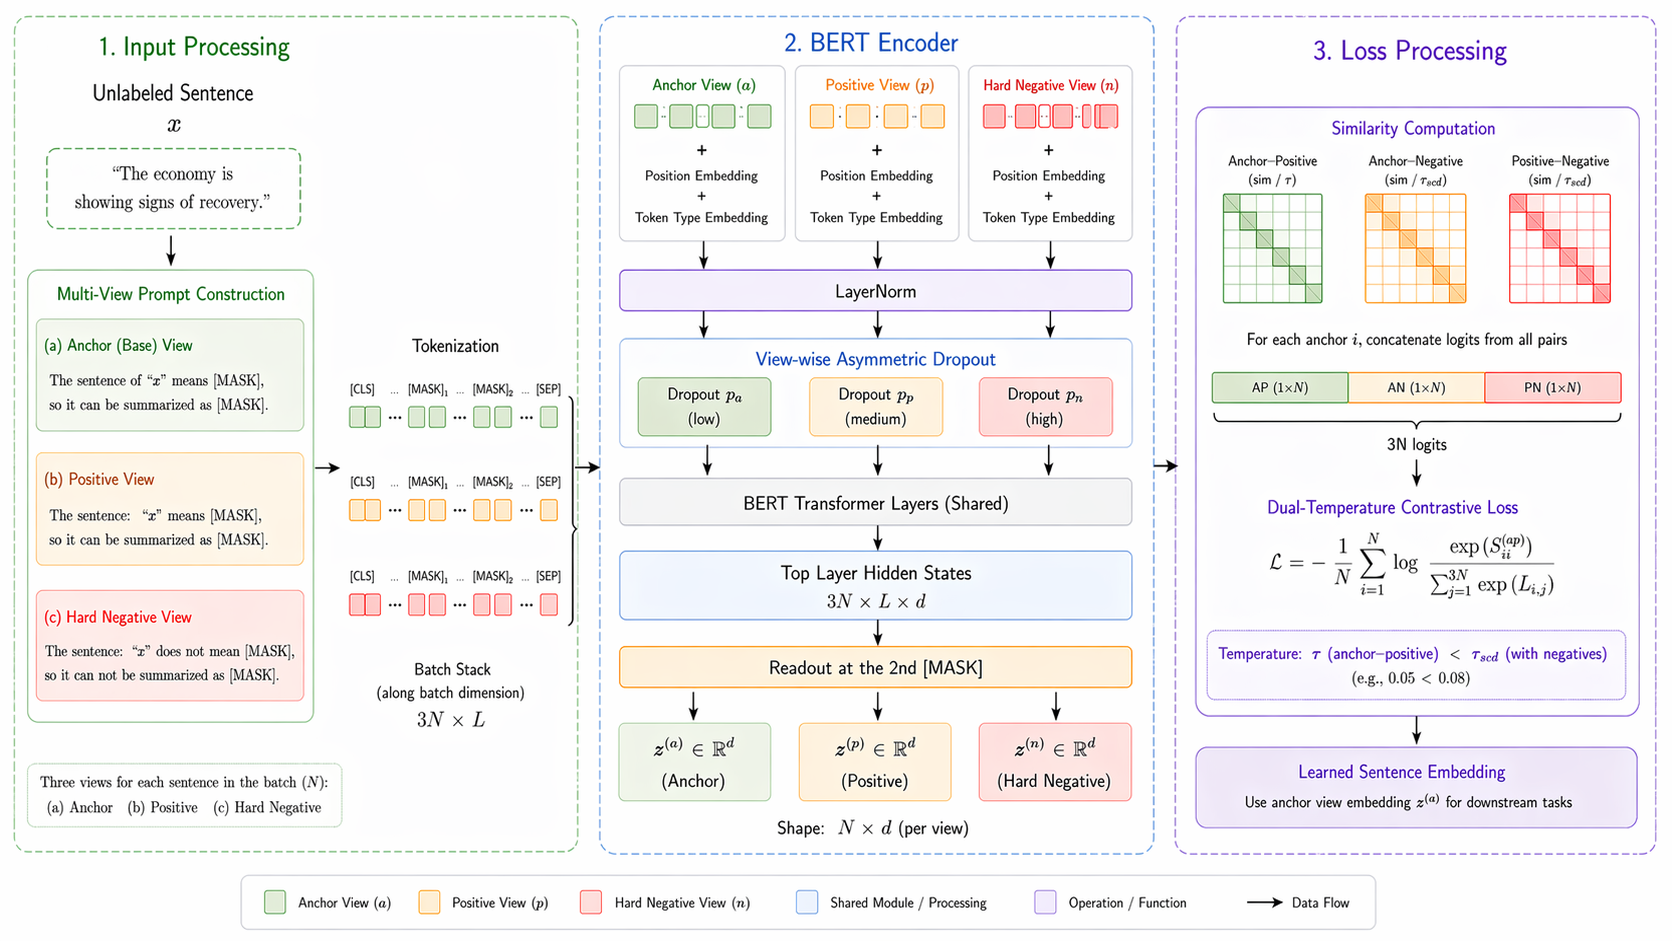
\includegraphics[width=.92\textwidth]{framework}
\caption{Overall architecture of MV-RaCL. For the same input sentence $x$, three prompt views (anchor, positive, and hard-negative) are first constructed; the three views are then fed into a weight-shared BERT encoder, and view-dependent asymmetric dropout is applied at the embedding layer; finally, the sentence representation is read from the second <MASK> position, and the model is trained end-to-end with a dual-temperature contrastive objective.}
\label{fig:framework}
\end{figure*}

To overcome this, the model must differentiate the distinct semantic functions---query, alignment, and rejection---assigned to different training views. We propose MV-RaCL, a novel framework that instantiates a unified View-Role Inductive Bias (VRIB). As illustrated in Fig.~\ref{fig:framework}, VRIB breaks the role-agnostic limitation across three progressive levels: signaling semantic roles at the input via three-view prompts (Section~\ref{subsec:prompts}), reinforcing these roles during encoding via view-dependent asymmetric dropout (Section~\ref{subsec:encoding}), and co-optimizing them through a dual-temperature hard-negative contrastive loss (Section~\ref{subsec:dt-loss}).


\subsection{Role Delineation via Three-View Prompts}
\label{subsec:prompts}

To explicitly delineate semantic roles at the input side without relying on external paraphrase corpora, we construct three distinct prompt views for each input sentence $x$: an anchor view, a positive view, and a hard-negative view. Their formal surface forms are detailed in Table~\ref{tab:prompts}.

\begin{table*}[!htbp]
\centering
\caption{Three-view prompt templates for anchor ($\tilde{x}^{(a)}$), positive ($\tilde{x}^{(p)}$), and hard-negative ($\tilde{x}^{(n)}$) roles.}
\label{tab:prompts}
\small
\setlength{\tabcolsep}{5pt}
\renewcommand{\arraystretch}{1.15}
\begin{tabular*}{\linewidth}{@{\extracolsep{\fill}}>{\raggedright\arraybackslash}p{0.17\textwidth}>{\centering\arraybackslash}p{0.11\textwidth}>{\raggedright\arraybackslash}p{0.66\textwidth}@{}}
\toprule
\textbf{Role} & \textbf{View} & \textbf{Prompt template} \\
\midrule
Anchor / Base & $\tilde{x}^{(a)}$ &
$\text{``The sentence of ''$x$'' means <MASK>,\allowbreak{} so it can be summarized as <MASK>.''}$ \\
Positive & $\tilde{x}^{(p)}$ &
$\text{``The sentence: ''$x$'' means <MASK>,\allowbreak{} so it can be summarized as <MASK>.''}$ \\
Hard-negative & $\tilde{x}^{(n)}$ &
$\text{``The sentence: ''$x$'' does not mean <MASK>,\allowbreak{} so it cannot be summarized as <MASK>.''}$ \\
\bottomrule
\end{tabular*}
\end{table*}

The Anchor view ($\tilde{x}^{(a)}$) embeds the original sentence into a chain-style ``key-point--summary'' context to highlight its core propositional content. The Positive view ($\tilde{x}^{(p)}$) utilizes a structurally similar template that differs only in surface wording, forming a natural anchor-positive alignment pair. Crucially, the Hard-negative view ($\tilde{x}^{(n)}$) employs a negation-based template, explicitly introducing opposing expressions like ``does not mean.'' This negation template serves as an explicit inductive bias, forcing a confusable, opposing semantic role at the input side. After tokenization, these three templates are concatenated and fed into the BERT encoder.

\subsection{Boundary Reinforcement via Asymmetric Encoding}
\label{subsec:encoding}

While standard BERT represents tokens as the sum of token, position, and segment embeddings:
\begin{equation}
\mathbf{e}_i = \mathbf{E}_{\mathrm{tok}}(x_i) + \mathbf{E}_{\mathrm{pos}}(i) + \mathbf{E}_{\mathrm{type}}(s_i)
\end{equation}
where $s_i$ denotes the token-type index, we deliberately avoid adding a learnable view-ID embedding. Instead, view-role information injected by the prompts is reinforced at the representation level through view-dependent asymmetric dropout.

Because the three views serve different semantic functions, their sensitivity to random perturbation varies. The anchor view requires relative stability ($p^{(a)}$) to anchor core semantics; the positive view tolerates moderate perturbation ($p^{(p)}$) to improve robustness; and the hard-negative view demands stronger perturbation ($p^{(n)}$) to suppress superficial shortcut alignments. Thus, during the single forward pass of the concatenated tensor $(3N, L, d)$, we apply independent dropout intensities satisfying $p^{(a)} < p^{(p)} < p^{(n)}$:
\begin{equation}
\mathbf{h}^{(v)} = \mathrm{Dropout}_v\bigl(\mathbf{e}^{(v)}\bigr), \quad p^{(a)} \,<\, p^{(p)} \,<\, p^{(n)}
\end{equation}

Finally, we extract the top-layer hidden state at the second <MASK> position as the focused sentence representation ($\mathbf{z}^{(a)}$, $\mathbf{z}^{(p)}$, and $\mathbf{z}^{(n)}$):
\begin{equation}
\mathbf{z}^{(v)} = f_\theta\bigl(\tilde{x}^{(v)}\bigr)_{\text{MASK}_2}
\end{equation}

\subsection{Gradient Redistribution via Dual-Temperature Objective}
\label{subsec:dt-loss}

Conventional InfoNCE objectives typically draw in-batch negatives and share a single temperature $\tau$ across all similarity terms. This uniform optimization struggles to separately calibrate the gradient demands for pulling positives closer versus pushing hard negatives apart.

MV-RaCL addresses this by explicitly placing the hard-negative representation in the softmax denominator and assigning an independent, larger temperature $\tau_{\mathrm{scd}}$ to similarity terms involving the negative view. As defined in Equations (\ref{eq:sim-groups})--(\ref{eq:sim-groups3}), we compute three groups of cosine similarities: $S^{(ap)}$, $S^{(an)}$, and $S^{(pn)}$.
\begin{align}
\label{eq:sim-groups}
S^{(ap)}_{ij} &= \mathrm{sim}\bigl(\mathbf{z}_i^{(a)},\, \mathbf{z}_j^{(p)}\bigr)\,/\,\tau \\
S^{(an)}_{ij} &= \mathrm{sim}\bigl(\mathbf{z}_i^{(a)},\, \mathbf{z}_j^{(n)}\bigr)\,/\,\tau_{\mathrm{scd}} \\
\label{eq:sim-groups3}
S^{(pn)}_{ij} &= \mathrm{sim}\bigl(\mathbf{z}_i^{(p)},\, \mathbf{z}_j^{(n)}\bigr)\,/\,\tau_{\mathrm{scd}}
\end{align}

\paragraph{Loss function.} For sample index $i$, we concatenate the three similarity rows $S^{(ap)}_{i,1:N}$, $S^{(an)}_{i,1:N}$, and $S^{(pn)}_{i,1:N}$ into a single logits vector $\mathbf{L}_i \in \mathbb{R}^{3N}$, with the diagonal entry $S^{(ap)}_{ii}$ acting as the logit of the correct class. The dual-temperature contrastive loss (Eq.~\ref{eq:loss}) concatenates these into a single logits vector.
\begin{equation}
\label{eq:loss}
\mathcal{L} = -\frac{1}{N}\sum_{i=1}^{N} \log \frac{\exp\bigl(S^{(ap)}_{ii}\bigr)}{\sum_{j=1}^{3N} \exp\bigl([\mathbf{L}_i]_{j}\bigr)}
\end{equation}

By setting $\tau_{\mathrm{scd}} > \tau$, the raw cosine similarity of hard negatives enters the softmax at a reduced magnitude. This gradient reweighting flattens the distribution over negative-view logits, attenuating overly strong gradient shocks that hard negatives would otherwise impose on anchor-positive alignment, while still providing a structured rejection signal. Consequently, this design achieves a soft redistribution of gradient mass between positive alignment and hard-negative rejection.

For sample $i$, let $Z_i = \sum_{j=1}^{3N} \exp([\mathbf{L}_i]_j)$ denote the partition function. The gradient of $\mathcal{L}$ with respect to the anchor--positive logit satisfies
\begin{equation}
\frac{\partial \mathcal{L}}{\partial S^{(ap)}_{ii}}
= -\frac{1}{N}\left(1 - \frac{\exp(S^{(ap)}_{ii})}{Z_i}\right),
\end{equation}
whereas for an anchor--negative logit $S^{(an)}_{ij}$ ($j \neq i$),
\begin{equation}
\frac{\partial \mathcal{L}}{\partial S^{(an)}_{ij}}
= \frac{1}{N}\,\frac{\exp(S^{(an)}_{ij})}{Z_i}.
\end{equation}
Because $S^{(an)}_{ij}$ is scaled by the larger temperature $\tau_{\mathrm{scd}}$, its raw cosine similarity enters the softmax at reduced magnitude relative to anchor--positive terms scaled by $\tau$. This \emph{gradient reweighting} attenuates hard-negative shocks on anchor--positive alignment while still keeping negative-view logits in the denominator---unlike SimCSE or CoT-BERT, which rely on a single $\tau$ and do not expose an explicit hard-negative view in the loss.

\begin{table}[!htbp]
\centering
\caption{View-Role-Aware Contrastive Training (MV-RaCL)}
\label{alg:mvracl}
\small
\setlength{\tabcolsep}{2pt}
\begin{tabular*}{\columnwidth}{@{\extracolsep{\fill}}>{\raggedright\arraybackslash}p{0.96\columnwidth}@{}}
\toprule
\textbf{Algorithm 1} View-Role-Aware Contrastive Training \\
\midrule
\textbf{Input:} Unlabeled corpus $\mathcal{D}$, BERT encoder $f_\theta$, batch size $N$, temperatures $\tau < \tau_{\mathrm{scd}}$, dropout rates $p^{(a)} < p^{(p)} < p^{(n)}$ \\
\textbf{Output:} Trained parameters $\theta$ \\
\addlinespace[2pt]
1. \textbf{for} each mini-batch $\{x_i\}_{i=1}^{N} \subset \mathcal{D}$ \textbf{do} \\
2.\quad \textbf{for} $i = 1$ to $N$ \textbf{do} build anchor, positive, and hard-negative prompts $\tilde{x}_i^{(a)}, \tilde{x}_i^{(p)}, \tilde{x}_i^{(n)}$ (Table~\ref{tab:prompts}) \\
3.\quad Concatenate three views; apply $\mathrm{Dropout}_{p^{(a/p/n)}}$ at the embedding layer; forward through $f_\theta$ \\
4.\quad Read out $\mathbf{z}_i^{(a)}, \mathbf{z}_i^{(p)}, \mathbf{z}_i^{(n)}$ from the second <MASK> slot \\
5.\quad Form $S^{(ap)}, S^{(an)}, S^{(pn)}$; build logits $\mathbf{L}_i \in \mathbb{R}^{3N}$ (Eqs.~(\ref{eq:sim-groups})--(\ref{eq:loss})) \\
6.\quad Minimize dual-temperature InfoNCE $\mathcal{L}$; update $\theta$ \\
7. \textbf{end for} \\
\bottomrule
\end{tabular*}
\end{table}

\begin{table*}[!htbp]
\centering
\caption{Mechanistic comparison of unsupervised BERT-base sentence encoders in Table~\ref{tab:main} (training-time design). Block~1: lightweight prompt methods without external data; Block~2: RankEncoder (external reference corpus; context only).}
\label{tab:mech-compare}
\footnotesize
\setlength{\tabcolsep}{4pt}
\renewcommand{\arraystretch}{1.12}
\begin{tabular*}{\linewidth}{@{\extracolsep{\fill}}>{\raggedright\arraybackslash}p{0.15\textwidth}*{6}{>{\raggedright\arraybackslash}p{0.12\textwidth}}@{}}
\toprule
\textbf{Design aspect} & \multicolumn{5}{c}{\textit{Block 1 --- Lightweight unsupervised prompt methods (no external data)}} & \textit{Block 2} \\
\cmidrule(lr){2-6}\cmidrule(lr){7-7}
 & \textbf{SimCSE} & \textbf{PromptBERT} & \textbf{ConPVP} & \textbf{CoT-BERT} & \textbf{MV-RaCL} & \textbf{RankEncoder} \\
\midrule
Prompt views & None & prompt template & Multi-prompt ensemble & CoT template & Three role templates & Prompt-based encoder \\
Role differentiation & No & No & No & No & VRIB: template + asym.\ dropout & No \\
Hard-negative in loss & In-batch only & In-batch only & In-batch only & In-batch only & Explicit $3N$ denominator & In-batch + rank align. \\
Temperature & Single $\tau$ & Single $\tau$ & Single $\tau$ & Single $\tau$ & $\tau$ + $\tau_{\mathrm{scd}}$ & Single $\tau$ \\
External resources & None & None & None & None & None & Reference corpus \\
\bottomrule
\end{tabular*}
\end{table*}

Algorithm~\ref{alg:mvracl} and Table~\ref{tab:mech-compare} summarize the full training pipeline and mechanistic differences across the encoders in Table~\ref{tab:main}.

%% ================================================================
%% 4. Experiments
%% ================================================================
\section{Experiments}
\label{sec:exp}

This section provides empirical validation for our proposed MV-RaCL framework. First, in Section~\ref{subsec:setup-exp}, we outline the experimental setup, including the evaluation benchmarks and implementation details. Following this, in Section~\ref{subsec:main}, we present the main results on composition-sensitive and general STS matching. Then, in Section~\ref{subsec:ablation}, we conduct an ablation study to confirm the contribution of each key component. Finally, in Sections~\ref{subsec:repr} and \ref{subsec:case}, we perform an in-depth representation-space analysis and case study to elucidate the underlying mechanisms that drive MV-RaCL's effectiveness.

\subsection{Experimental Setup}
\label{subsec:setup-exp}

We evaluate sentence representations using the SentEval~\cite{senteval} toolkit. The general STS benchmark consists of STS12--STS16 and STS-Benchmark (six tasks in total); we report Spearman's rank correlation on the test sets, denoted as $\rho \times 100$. In addition, SICK-Relatedness (SICK-R)~\cite{sick} is used to assess composition-sensitive matching involving negation, word order, quantification, and predicate substitution. The overall protocol follows the public setting of SimCSE and subsequent work; STS12--16, STS-B, and SICK-R follow standard SentEval splits. We evaluate MV-RaCL not to claim superiority on all STS tasks, but to test whether introducing a role-aware mechanism yields \emph{selective compositional sharpening}, through a four-stage evidence chain: headline benchmark gains on SICK-R, controlled ablations, representation-space geometry, and per-phenomenon case spot-checks, with STS-B serving throughout as a general-matching guardrail.

For controlled comparison, all main experiments are restricted to an unsupervised, BERT-base ($\sim$110M parameters) setting; we do not use supervised NLI data, external teacher distillation, or auxiliary reference corpora. Methods that depend on large-scale supervised data, long-context multilingual pre-training, or large language models (e.g., E5~\cite{e5}, mGTE~\cite{gte}) fall outside this comparable regime and are not listed in the main table. Our baselines include GloVe (averaged word vectors), USE, BERT-flow, BERT-whitening, IS-BERT~\cite{isbert}, ConSERT~\cite{consert}, SimCSE~\cite{simcse}, DCLR~\cite{dclr}, ArcCSE~\cite{arccse}, ESimCSE~\cite{esimcse}, DiffCSE~\cite{diffcse}, PCL~\cite{pcl}, PromCSE~\cite{promcse}, PromptBERT~\cite{promptbert}, ConPVP~\cite{conpvp}, and RankEncoder~\cite{rankencoder}, with CoT-BERT~\cite{cotbert} serving as our direct baseline.

Training is initialized from HuggingFace's bert-base-uncased. The unsupervised corpus consists of approximately 1M sentences randomly sampled from English Wikipedia, identical to the data used by SimCSE. We use the AdamW optimizer with a peak learning rate of $2\times 10^{-5}$, a linear-decay schedule, and a warmup ratio of $0.05$; the batch size is $64$ and we train for $3$ epochs, selecting the best checkpoint on the STS-B development set. The contrastive temperatures are set to $\tau = 0.05$ and $\tau_{\mathrm{scd}} = 0.08$ (Section~\ref{subsec:dt-loss}); the three view-dependent embedding dropout probabilities are set to $p^{(a)} = 0.10$, $p^{(p)} = 0.15$, and $p^{(n)} = 0.35$ (Section~\ref{subsec:encoding}). At evaluation time we follow the same sentence-representation extraction protocol as CoT-BERT.

Table~\ref{tab:main} reports only SICK-R and STS-B: SICK-R is the \emph{primary} metric aligned with our VRIB design (compositional semantics, negation, and hard negatives), whereas STS-B serves as a \emph{guardrail} for general semantic matching, keeping the headline comparison readable at a glance.

\subsection{Main Results}
\label{subsec:main}

Table~\ref{tab:main} compares lightweight unsupervised prompt methods (Block~1) and, for context, a ranking-augmented system that requires an external reference corpus (Block~2).

\begin{table*}[!htbp]
\centering
\caption{Spearman correlations ($\rho \times 100$) on \textbf{SICK-R} (primary: compositional/negation-related relatedness) and \textbf{STS-B} (general STS guardrail). \textbf{Block~1} compares methods without external data; \textbf{Block~2} reports RankEncoder for context. \textbf{Bold}: best \emph{within Block~1} per column.}
\label{tab:main}
\small
\setlength{\tabcolsep}{6pt}
\begin{tabular*}{\linewidth}{@{\extracolsep{\fill}}lcc@{}}
\toprule
Method & \textbf{SICK-R} & STS-B \\
\midrule
\multicolumn{3}{@{}l@{}}{\textit{Block 1 --- Lightweight unsupervised prompt methods (no external data)}} \\
\addlinespace[2pt]
SimCSE~\cite{simcse} & 72.23 & 76.85 \\
PromptBERT~\cite{promptbert} & 69.87 & 81.60 \\
ConPVP~\cite{conpvp} & 73.38 & 80.82 \\
\rowcolor{blue!8}
CoT-BERT~\cite{cotbert} & 71.41 & \textbf{82.40} \\
\rowcolor{blue!8}
MV-RaCL (Ours) & \cellcolor{green!12}\textbf{74.65} & 81.75 \\
\addlinespace[2pt]
$\Delta$ (Ours $-$ CoT-BERT) & +3.24 & $-$0.65 \\
\midrule
\multicolumn{3}{@{}l@{}}{\textit{Block 2 --- Ranking-augmented (external reference corpus; context only)}} \\
\addlinespace[2pt]
RankEncoder~\cite{rankencoder} & 75.78 & 81.55 \\
\bottomrule
\end{tabular*}

\vspace{4pt}
{\footnotesize\raggedright
\noindent\textit{Note.} (1)~Primary Block~1 gain: SICK-R \textbf{+3.24} (71.41$\rightarrow$74.65) vs.\ CoT-BERT; STS-B \textbf{$-$0.65}. (2)~Best Block~1 SICK-R without external resources: \textbf{74.65}. (3)~Block~2 is not directly comparable (external reference corpus). (4)~Bold applies within Block~1 only.\par
}
\end{table*}

Table~\ref{tab:main} shows that MV-RaCL delivers a targeted and significant gain on compositional relatedness. Compared with the direct baseline CoT-BERT, SICK-R improves from $71.41$ to $74.65$ ($+3.24$, $+4.5\%$ relative). These results are highly encouraging: within Block~1, MV-RaCL achieves the best SICK-R score (74.65 $>$ ConPVP 73.38 $>$ SimCSE 72.23 $>$ CoT-BERT 71.41). This provides compelling evidence that the View-Role Inductive Bias (VRIB) effectively resolves the role-agnostic bottleneck. More impressively, on STS-B, MV-RaCL remains within $0.65$ points of CoT-BERT ($81.75$ vs.\ $82.40$), indicating a true \emph{selective compositional sharpening} rather than a trivial uniform similarity inflation.

Furthermore, while RankEncoder (Block~2) achieves a high score ($75.78$), it heavily depends on an external reference corpus. MV-RaCL completes end-to-end training within a single BERT-base encoder without introducing any external teachers or corpora, yet still approaches RankEncoder's performance on SICK-R. This underscores the simplicity and effectiveness of our internal role-differentiation strategy.

\subsection{Ablation Study}
\label{subsec:ablation}

This section adopts a controlled-variable design to systematically analyze the contribution of three key components: role differentiation via the three-view prompts, the transition from nearly symmetric to asymmetric embedding dropout, and the dual-temperature contrastive objective that strengthens hard-negative supervision. Table~\ref{tab:ablation} compares the SICK-R performance of these variants under a unified protocol, taking CoT-BERT as the starting point.

\begin{table*}[!htbp]
\centering
\caption{Ablation variants and SICK-R results. The parameter column reports the three-view embedding dropout values and the temperature setting; numbers are Spearman correlations ($\rho \times 100$).}
\label{tab:ablation}
\small
\setlength{\tabcolsep}{4pt}
\begin{tabular*}{\linewidth}{@{\extracolsep{\fill}}lcccc@{}}
\toprule
Variant & $p^{(a)}/p^{(p)}/p^{(n)}$ & $\tau$ & $\tau_{\mathrm{scd}}$ & SICK-R \\
\midrule
Base CoT-BERT                & ---              & ---  & ---  & 70.09 \\
+ Indep.\ emb.\ dropout      & $0.10/0.10/0.10$ & 0.05 & 0.05 & 70.94 \\
+ Asym.\ emb.\ dropout       & $0.10/0.15/0.35$ & 0.05 & 0.05 & 73.10 \\
Full model (MV-RaCL)         & $0.10/0.15/0.35$ & 0.05 & 0.08 & 74.65 \\
\bottomrule
\end{tabular*}
\end{table*}

We note that the \texttt{Base CoT-BERT} entry in Table~\ref{tab:ablation} serves only as an internal reference point under the same ablation protocol : its training and evaluation are re-implemented in this work to ensure that all variants share comparable conditions. As a consequence, its absolute value differs from the CoT-BERT main-table number in Table~\ref{tab:main} (which is taken from the original paper), and the two should not be compared entry-by-entry. The focus of this section is the relative-gain trend under the unified protocol.

As shown in Table~\ref{tab:ablation}, SICK-R increases monotonically as the components are added: from the baseline $70.09$ to $70.94$, $73.10$, and finally $74.65$ for the full model. Specifically, independent embedding dropout equips the three views with mutually independent perturbation channels, providing the necessary structural foundation for subsequent role differentiation; asymmetric dropout further introduces view-dependent perturbation strength, sharpening the model's sensitivity to compositional semantic differences; and the dual-temperature objective uses differentiated temperatures to strengthen hard-negative supervision, contributing the largest single gain. These results indicate that the three key designs exhibit a clear progressive and complementary effect on SICK-R, and jointly support the full model's superior performance on composition-sensitive matching.

\subsection{Representation-Space Analysis}
\label{subsec:repr}

As demonstrated above, MV-RaCL excels in composition-sensitive text matching. In this subsection, we further explore the reasons behind this effectiveness by analyzing the geometry of the representation space.

\subsubsection{Alignment and Uniformity}
\label{subsec:au}

Following the analytical framework of Wang and Isola~\cite{alignment}, we estimate the alignment loss $\ell_{\mathrm{align}}$ and the uniformity loss $\ell_{\mathrm{uniform}}$ on the SICK-R test set, in order to characterize the geometry of the representation space and to help interpret performance differences on compositional relatedness. The two metrics are defined as
\begin{equation}
\ell_{\mathrm{align}}
=
\mathbb{E}_{(x,x^{+})\sim p_{\mathrm{pos}}}
\left\lVert f(x)-f(x^{+}) \right\rVert_2^{2}
\end{equation}
\begin{equation}
\ell_{\mathrm{uniform}}
=
\log \mathbb{E}_{x,y\sim p_{\mathrm{data}}}
\exp\!\left(-2\left\lVert f(x)-f(y) \right\rVert_2^{2}\right)
\end{equation}
Both metrics follow the standard scalar definitions in the sentence representation literature, with lower being better. To remain consistent with the SICK-R evaluation, $\ell_{\mathrm{align}}$ averages over all sentence pairs whose human-annotated relatedness is at least $4$, while $\ell_{\mathrm{uniform}}$ is estimated by random sampling of sentence pairs from the deduplicated set of test-set sentences under a fixed random seed.

\begin{table}[!htbp]
\centering
\caption{Alignment and Uniformity on the SICK-R test set for Base CoT-BERT and Full model (MV-RaCL); lower is better.}
\label{tab:au}
\begin{tabular}{lcc}
\toprule
Variant & Alignment & Uniformity \\
\midrule
Base CoT-BERT        & 0.1259 & $-1.6203$ \\
Full model (MV-RaCL) & 0.1181 & $-1.4267$ \\
\bottomrule
\end{tabular}
\end{table}

As shown in Table~\ref{tab:au}, while SICK-R Spearman improves from $70.09$ to $74.65$, $\ell_{\mathrm{align}}$ decreases from $0.1259$ to $0.1181$, a relative reduction of about $6.2\%$, indicating that highly related positive pairs are pulled closer in the representation space, consistent with the observed gains in compositional relatedness. At the same time, $\ell_{\mathrm{uniform}}$ rises from $-1.6203$ to $-1.4267$, indicating that the representation distribution slightly deviates from the optimum global uniformity. This phenomenon is consistent with the well-known alignment--uniformity trade-off: when the model places more emphasis on multi-view role modeling and hard-negative discrimination, gains in intra-class alignment do not necessarily translate into simultaneous improvements in global uniformity. These geometric scalars are therefore best regarded as complementary explanations of downstream task results, rather than as substitutes for indicators such as SICK-R.

\subsubsection{Cosine Distribution of Positives and Hard Negatives}
\label{subsec:cosine-dist}

To further examine the model's separation behavior in composition-sensitive discrimination, we compute on the SICK-R test set the cosine-similarity distributions of (i) the high-relatedness positive subset and (ii) a hard-negative subset constructed at evaluation time, and we visualize them as histograms for different training variants (Fig.~\ref{fig:cosine-dist}). Studying the conditional distributions of these two subsets answers two questions more directly than analyzing all sentence pairs jointly: whether highly related samples are stably concentrated in the high-cosine region, and whether superficially confusable but semantically dissimilar samples can be separated from positives. Note that the hard-negative subset here is defined by an operational rule of the evaluation protocol---requiring both low human relatedness and high token-level Jaccard overlap---so that, while it echoes the hard-negative view constructed by templates during training at the phenomenon level, the two are not strictly identical.

\begin{figure*}[!htbp]
\centering
\subfloat[Base CoT-BERT]{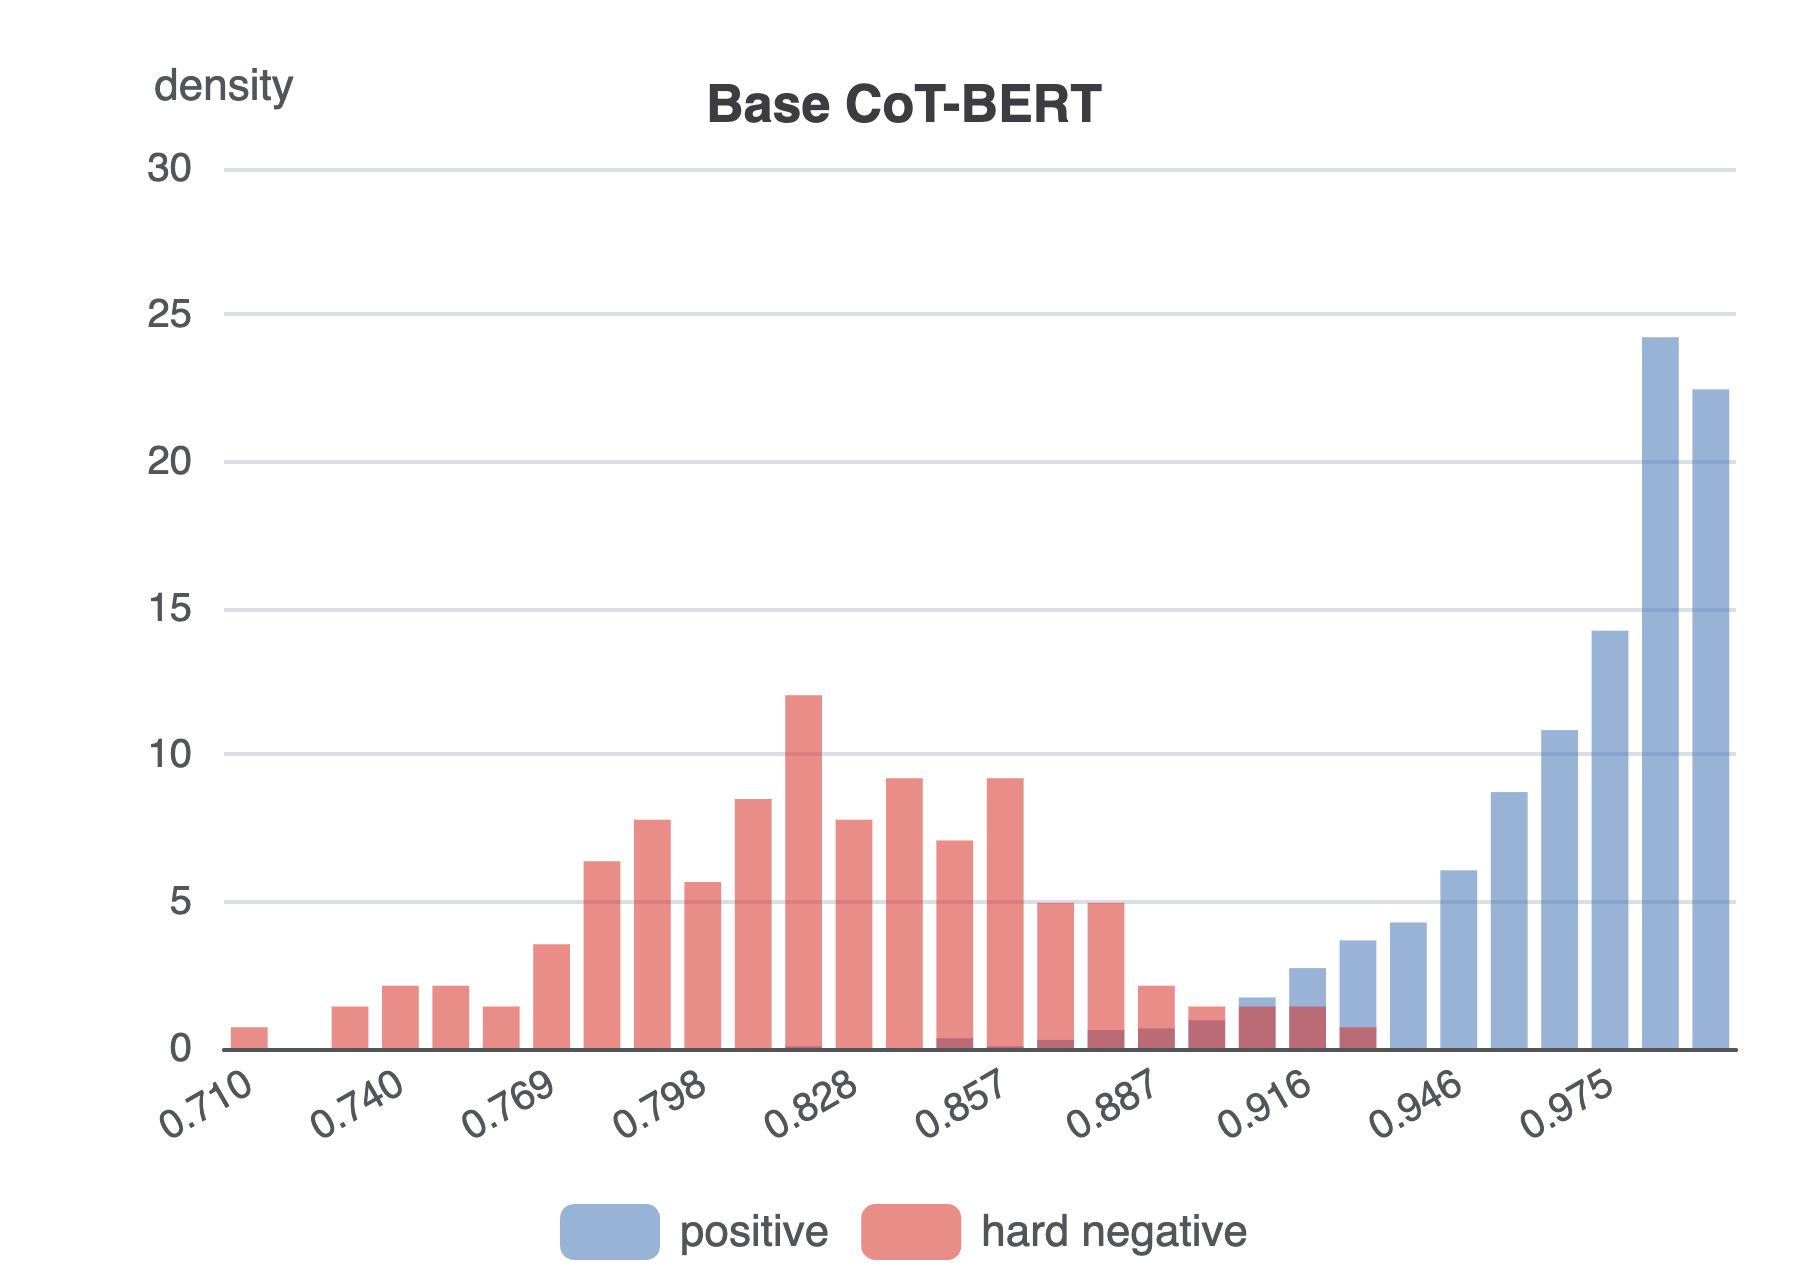
\includegraphics[width=0.46\linewidth]{his_base_cot}\label{fig:cos-base}}
\hfill
\subfloat[Full model (MV-RaCL)]{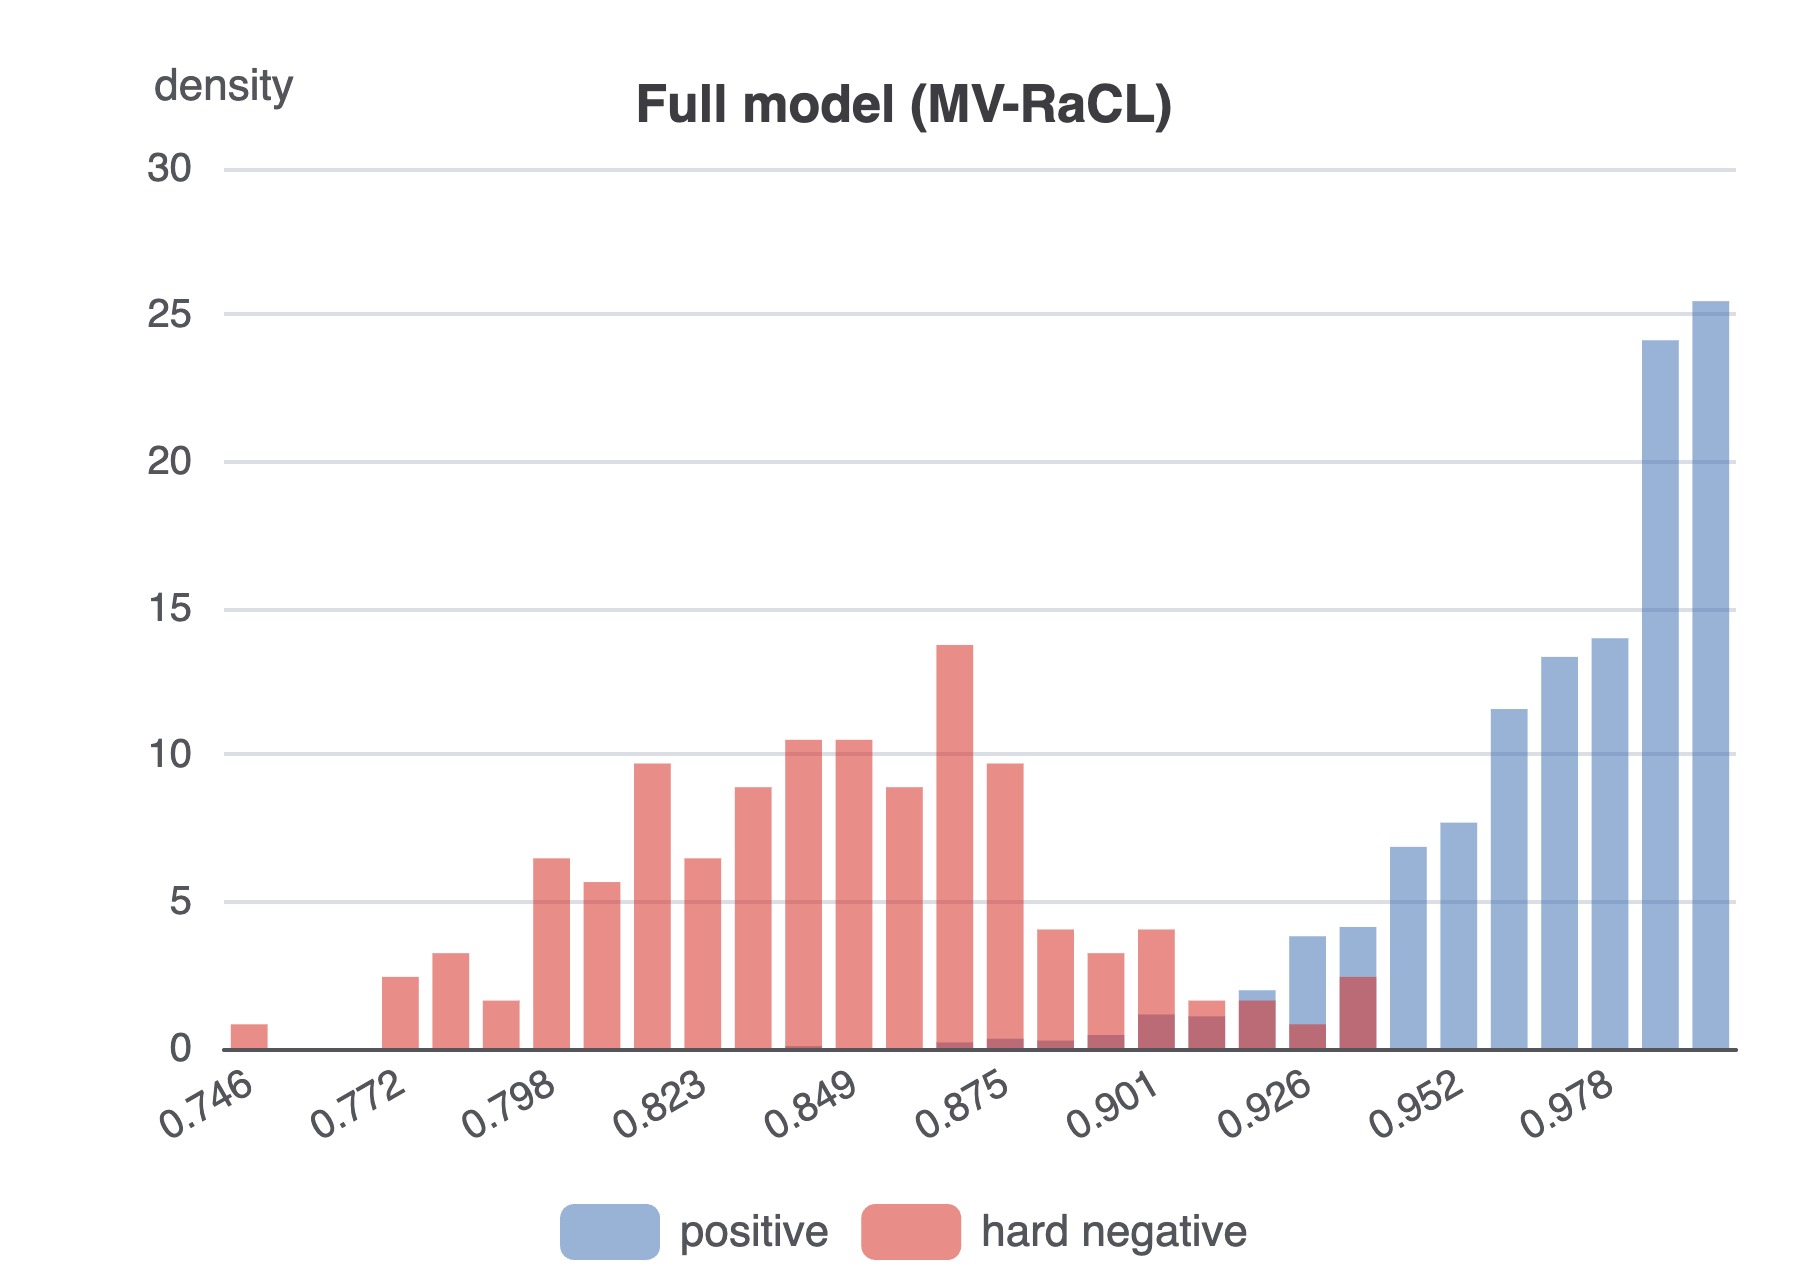
\includegraphics[width=0.46\linewidth]{his_full_model}\label{fig:cos-full}}
\caption{Cosine distributions of positives and hard negatives on the SICK-R test set. Blue: positive subset; red: hard-negative subset. Compared with the baseline, MV-RaCL exhibits stronger concentration of positives at high cosine values, while the overlap between hard negatives and positives remains largely confined to the intermediate transition region rather than intruding into the highest-cosine range.}
\label{fig:cosine-dist}
\end{figure*}

The analysis follows the same SICK-R evaluation pipeline---identical sentence-representation extraction, $L_2$ normalization, and pairwise cosine computation. The positive subset is defined as sentence pairs with human relatedness $\geq 4$; the hard-negative subset consists of pairs with human relatedness $\leq 2$ and token-level Jaccard overlap $\geq \tau_{\mathrm{jac}}$, where the main setting takes $\tau_{\mathrm{jac}}=0.25$. When the size of a given subset is too large, we randomly sample at most $K$ pairs per subset under a fixed random seed for plotting. Histograms use density on the y-axis, the number of bins is denoted by $B$, and all panels share the same y-axis range to allow comparison across variants.

In Fig.~\ref{fig:cosine-dist}, both models concentrate positives at high cosine values and hard negatives at lower-to-mid cosine values. Compared with the baseline, the full MV-RaCL pushes positives to higher cosine values more sharply, while the overlap between hard negatives and positives remains restricted to the middle transition region and does not encroach on the top-cosine range. This indicates that the main effect of our method is to tighten positive aggregation in the high-cosine zone and to prevent hard negatives from entering high-similarity regions, rather than to simply translate all negatives toward lower cosine values. The phenomenon is consistent with the SICK-R gain reported in Table~\ref{tab:ablation} and the alignment improvement in Table~\ref{tab:au}, and together they support the joint contribution of multi-view role modeling, asymmetric embedding dropout, and the dual-temperature objective. Fig.~\ref{fig:cosine-dist} should be regarded as complementary evidence and is not intended to substitute for the main quantitative results.

\subsubsection{Pair-Level Correspondence between Human Relatedness and Predicted Cosine}
\label{subsec:scatter}

Complementing the distribution-level evidence in Section~\ref{subsec:cosine-dist}, we examine, at the level of individual sentence pairs, how closely the predicted cosine similarity tracks human-annotated relatedness. On the SICK-R test set, each pair is encoded by the full MV-RaCL model and read out at two positions---the <CLS> token and the second <MASK> (MASK2)---following the same SentEval-style extraction protocol used for our main results (Section~\ref{subsec:setup-exp}); the resulting cosines are plotted against the corresponding human relatedness scores in Fig.~\ref{fig:scatter}.

\begin{figure*}[!htbp]
\centering
\subfloat[Readout from <CLS>]{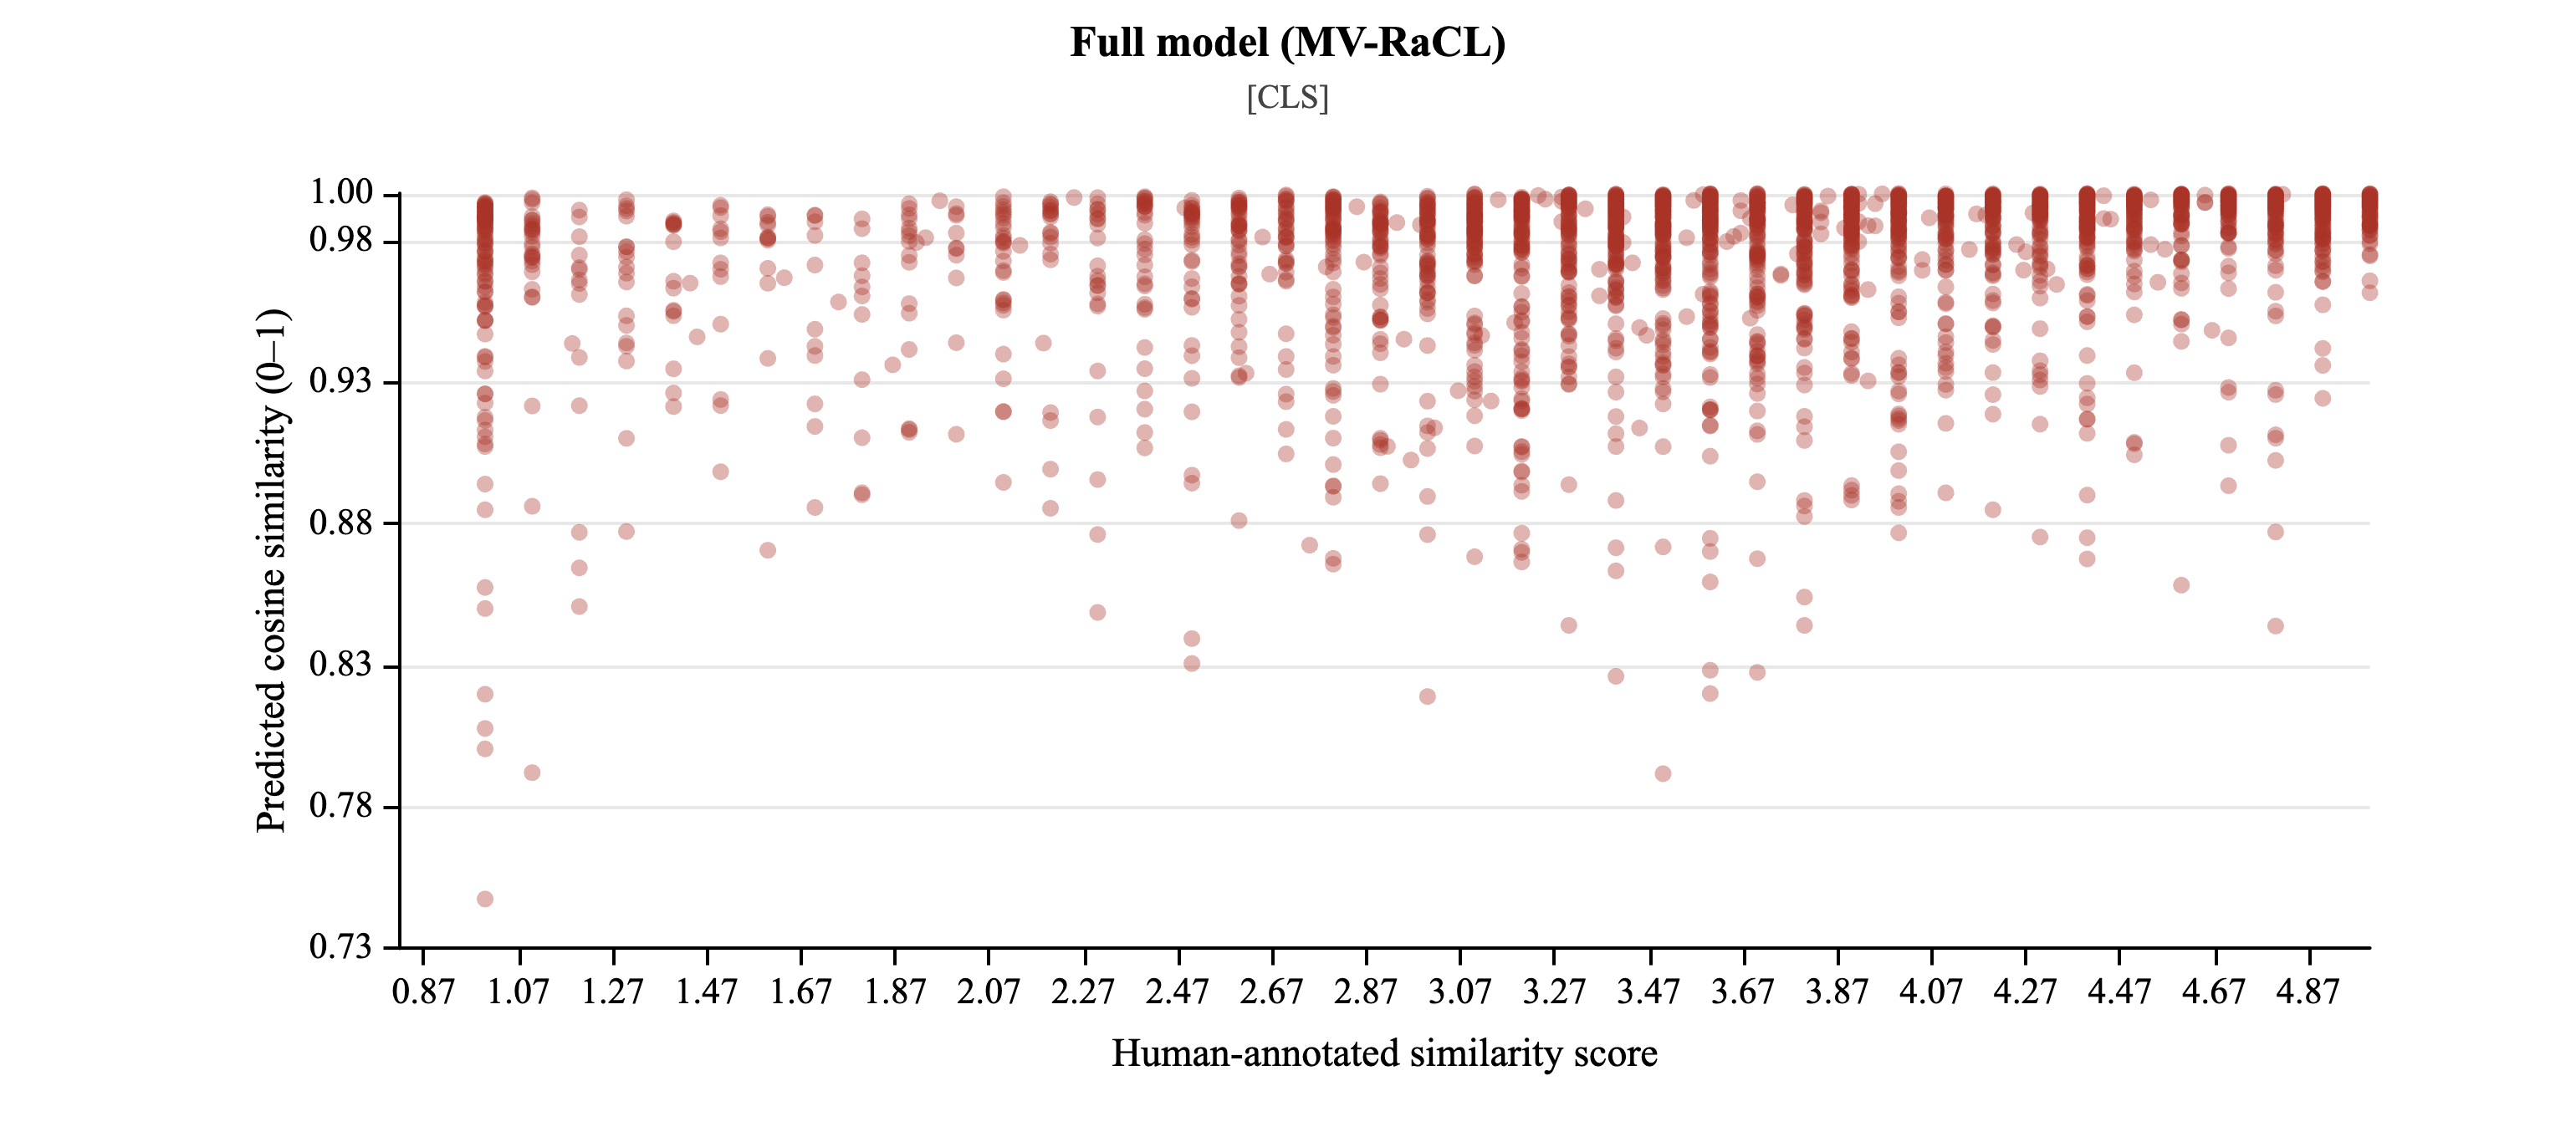
\includegraphics[width=0.46\linewidth]{cls_scatter}\label{fig:scatter-cls}}
\hfill
\subfloat[Readout from the second <MASK> (MASK2)]{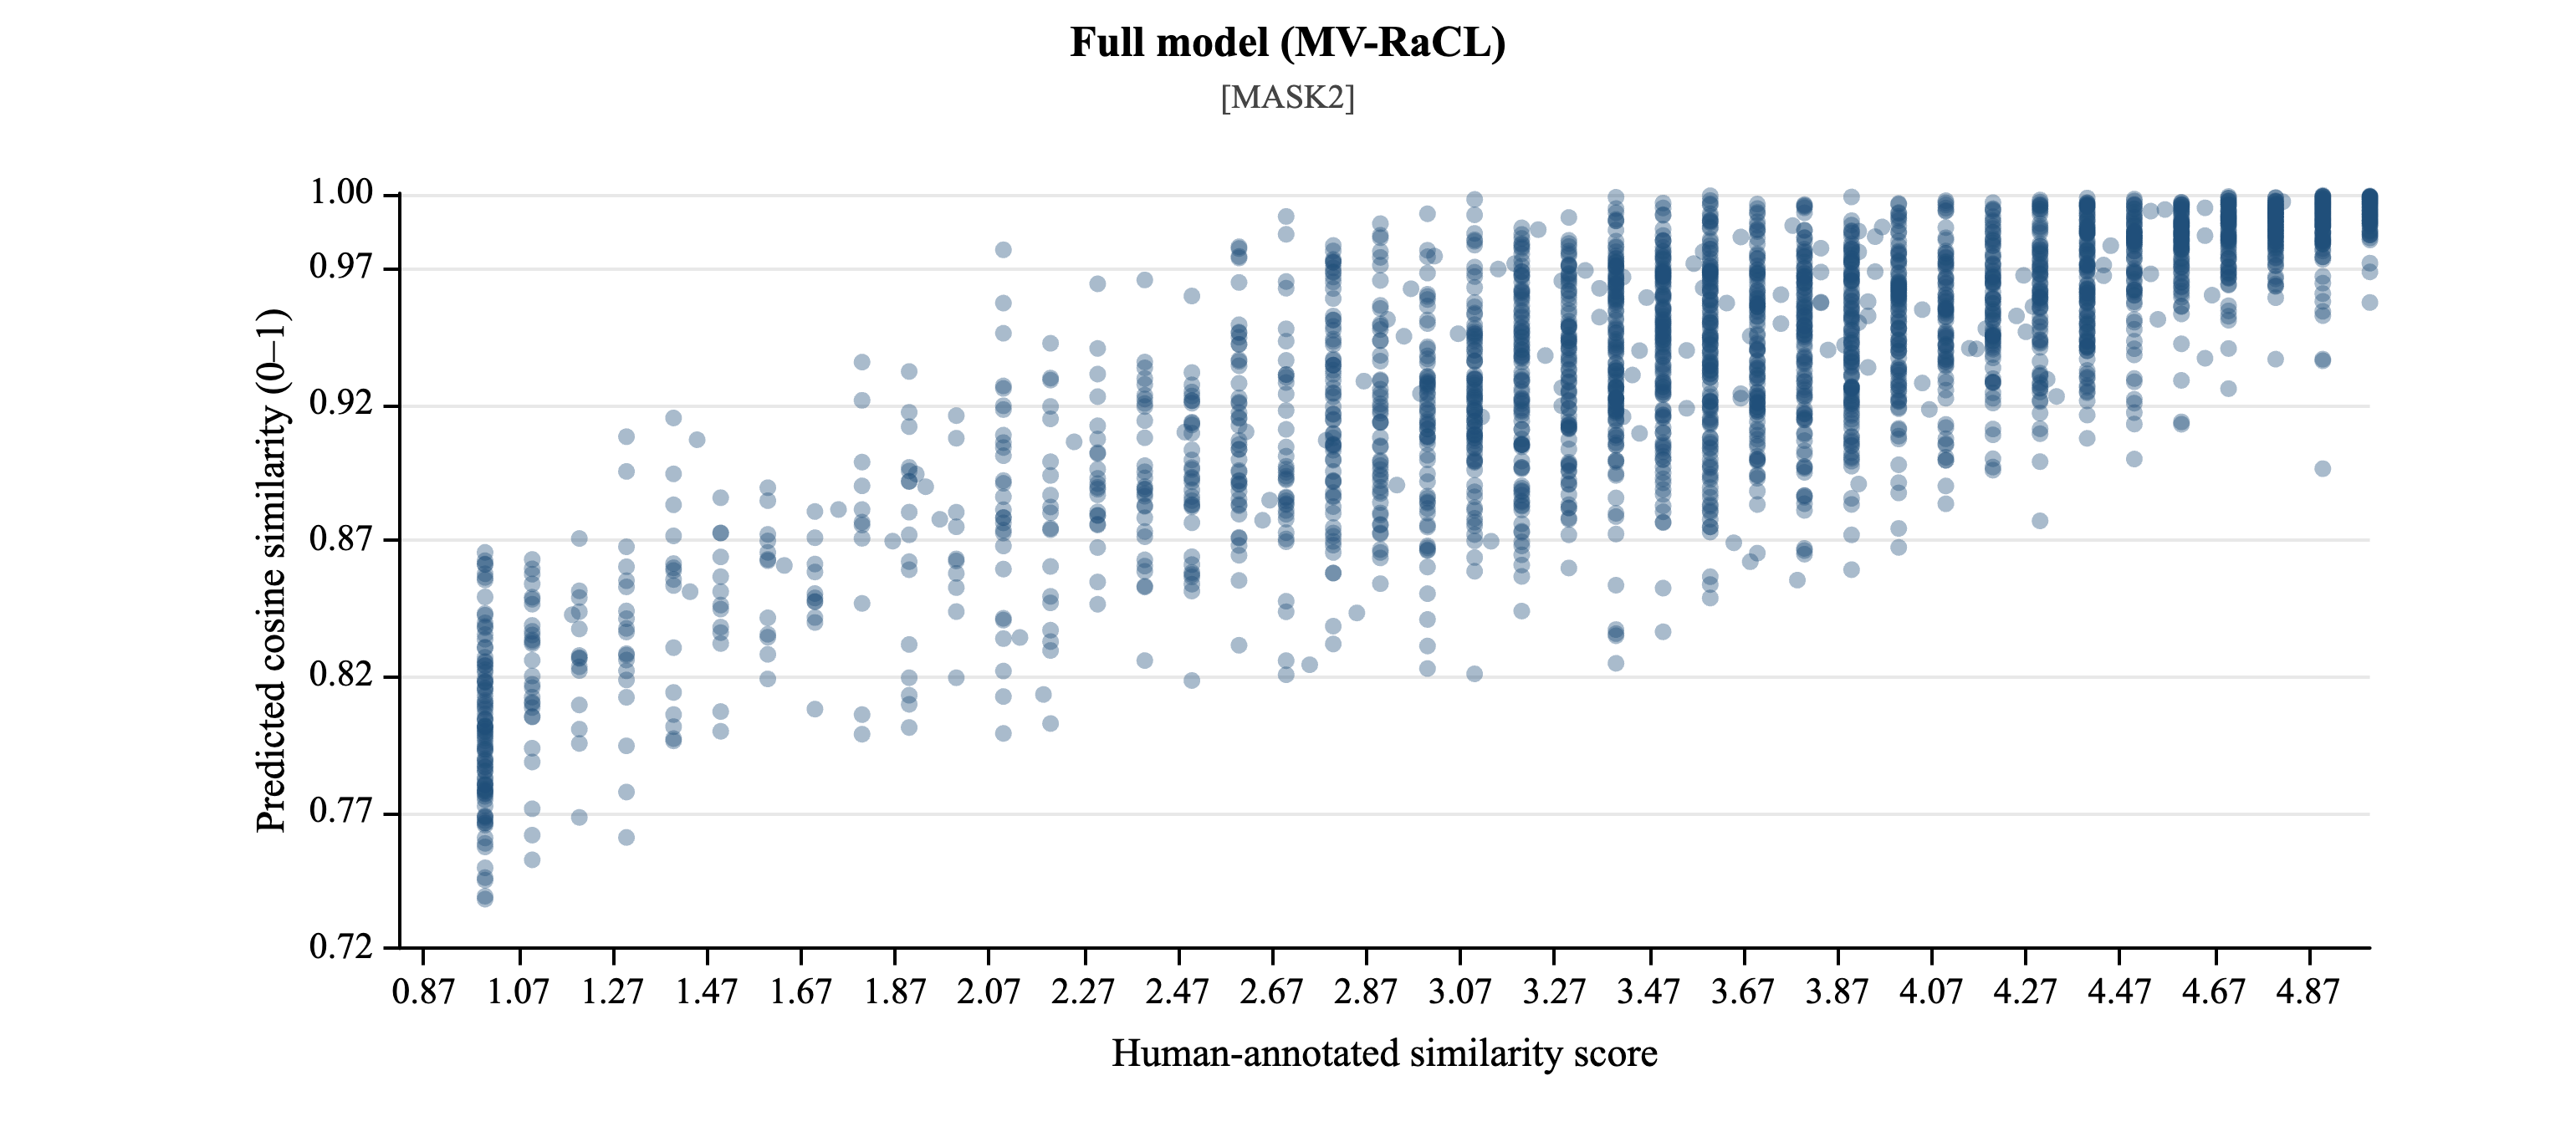
\includegraphics[width=0.46\linewidth]{mask_scatter}\label{fig:scatter-mask}}
\caption{Pair-level correspondence between human-annotated relatedness (x-axis) and the cosine similarity predicted by the full MV-RaCL model (y-axis) on the SICK-R test set, evaluated with sentence vectors read from (a) the <CLS> token and (b) the second <MASK> (MASK2). The MASK2 readout shows a substantially tighter monotonic association with human relatedness than the <CLS> readout, whose points cluster in a narrow high-cosine band. The vertical banding reflects the discrete relatedness scale of SICK-R rather than the embedding geometry.}
\label{fig:scatter}
\end{figure*}

Two observations emerge. First, the <CLS> readout collapses into a narrow high-cosine band that is largely insensitive to human judgement, consistent with the well-documented anisotropy of the raw <CLS> space~\cite{kurz2026tacl}. Second, the MASK2 readout exhibits a clear monotonic relationship: predicted cosine values increase steadily with human relatedness, and their dispersion narrows toward the high-relatedness end, so that highly related pairs concentrate near the top of the cosine scale while weakly related pairs remain distributed across the low- to mid-cosine range. The vertical banding common to both panels reflects only the discrete relatedness scale of SICK-R and is not a property of the embeddings. Taken together with the distribution-level evidence in Fig.~\ref{fig:cosine-dist}, these pair-level patterns provide direct empirical support for reading out sentence representations from the second <MASK> position (Section~\ref{subsec:encoding}).

\subsection{Case Analysis and Discussion}
\label{subsec:case}

Beyond the geometric properties of the representation space, this subsection provides a more granular inspection of MV-RaCL's behavior. We first examine typical sentence pairs...

\subsubsection{Typical Sentence Pairs}

General contrastive sentence representations often exhibit insufficient discriminative resolution under settings involving compositional semantics, negation, and hard negatives. To compare the direct baseline CoT-BERT and MV-RaCL at pair-level granularity, we fix the same set of sentence pairs from the SICK-R test set and, under the same sentence-representation protocol used in our main experiments, report the predicted cosine $\cos_{\mathrm{pred}}$ produced by each model.

\begin{table*}[!htbp]
\centering
\caption{Examples from the SICK-R test set with low human relatedness, where MV-RaCL's $\cos_{\mathrm{pred}}$ is strictly lower than CoT-BERT's. Type: H = hard-negative; N = negation; C = compositional/ambiguous.}
\label{tab:cases}
\small
\setlength{\tabcolsep}{2pt}
\renewcommand{\arraystretch}{1.05}
\begin{tabular}{p{0.27\textwidth}p{0.27\textwidth}cccc}
\toprule
Sentence A & Sentence B & Type & Human & cos (CoT-BERT) & cos (Ours) \\
\midrule
A man is riding the horse & A man is riding a motorbike & H & 2.40 & 0.9358 & 0.9258 \\
A boy is throwing away a calendar & A boy is looking at a calendar & H & 2.40 & 0.9349 & 0.9227 \\
A big city is begging for men and money holders & A man in a big city is holding a sign and begging for money & H & 2.40 & 0.9354 & 0.9276 \\
A brown dog is jumping in the air & A brown dog is sitting down & H & 2.50 & 0.9272 & 0.9159 \\
The woman is poking a potato & The woman is not poking holes in the potato & N & 2.40 & 0.9677 & 0.9380 \\
Not everyone is able to walk a lion & A lion is pacing tiredly in a pen & N & 2.30 & 0.8774 & 0.8490 \\
There is no boy wearing red shorts jumping into a paddling pool & A young boy wearing a red swimsuit is jumping into a blue kiddies pool & N & 2.20 & 0.9490 & 0.9217 \\
There is no man running, jumping and kicking near a vending machine & Three men are jumping off a wall & N & 2.00 & 0.8805 & 0.8551 \\
The windows are being cleaned by a man & The man has a window of time to clean himself & C & 1.75 & 0.9171 & 0.8838 \\
A baby rhino is following an adult rhino & A mother is giving the baby a pen with a walking rhino on it & C & 2.10 & 0.8992 & 0.8752 \\
A woman in a black dress is pulling a cart and is standing in front of two men who are seated on a park bench & A lady is dressed in black and is carrying a white cross & C & 2.50 & 0.8856 & 0.8664 \\
The man is driving a car & The man has a window of time to clean himself & C & 1.60 & 0.8152 & 0.7990 \\
\bottomrule
\end{tabular}
\end{table*}

The examples in Table~\ref{tab:cases} are all drawn from sentence pairs with low human relatedness ($\leq 2.5$). Pairs are first heuristically classified as: (H) hard negatives, (N) negation-related, or (C) compositional/ambiguous; if a sentence contains an explicit negation marker, it is preferentially assigned to N rather than H. Within H, we further prefer pairs with high token-level Jaccard overlap (about $0.40$--$0.57$ in this table) to expose ``high surface overlap, semantically dissimilar'' pressure cases. From each category, we select four pairs in which MV-RaCL's $\cos_{\mathrm{pred}}$ is strictly lower than the baseline's, yielding $12$ pairs in total. They illustrate that, on weakly related or unrelated pairs, MV-RaCL is able, on a case-by-case basis, to further suppress similarity estimates that should not be high. We emphasize that the Spearman result in Table~\ref{tab:ablation} and the distributional statistics in Section~\ref{subsec:cosine-dist} remain the primary basis for our conclusions; Table~\ref{tab:cases} only provides a category-balanced qualitative illustration and does not bear the burden of global inference.

\subsubsection{General STS vs.\ SICK-R: Cross-Metric Asynchrony}

\begin{figure*}[!htbp]
\centering
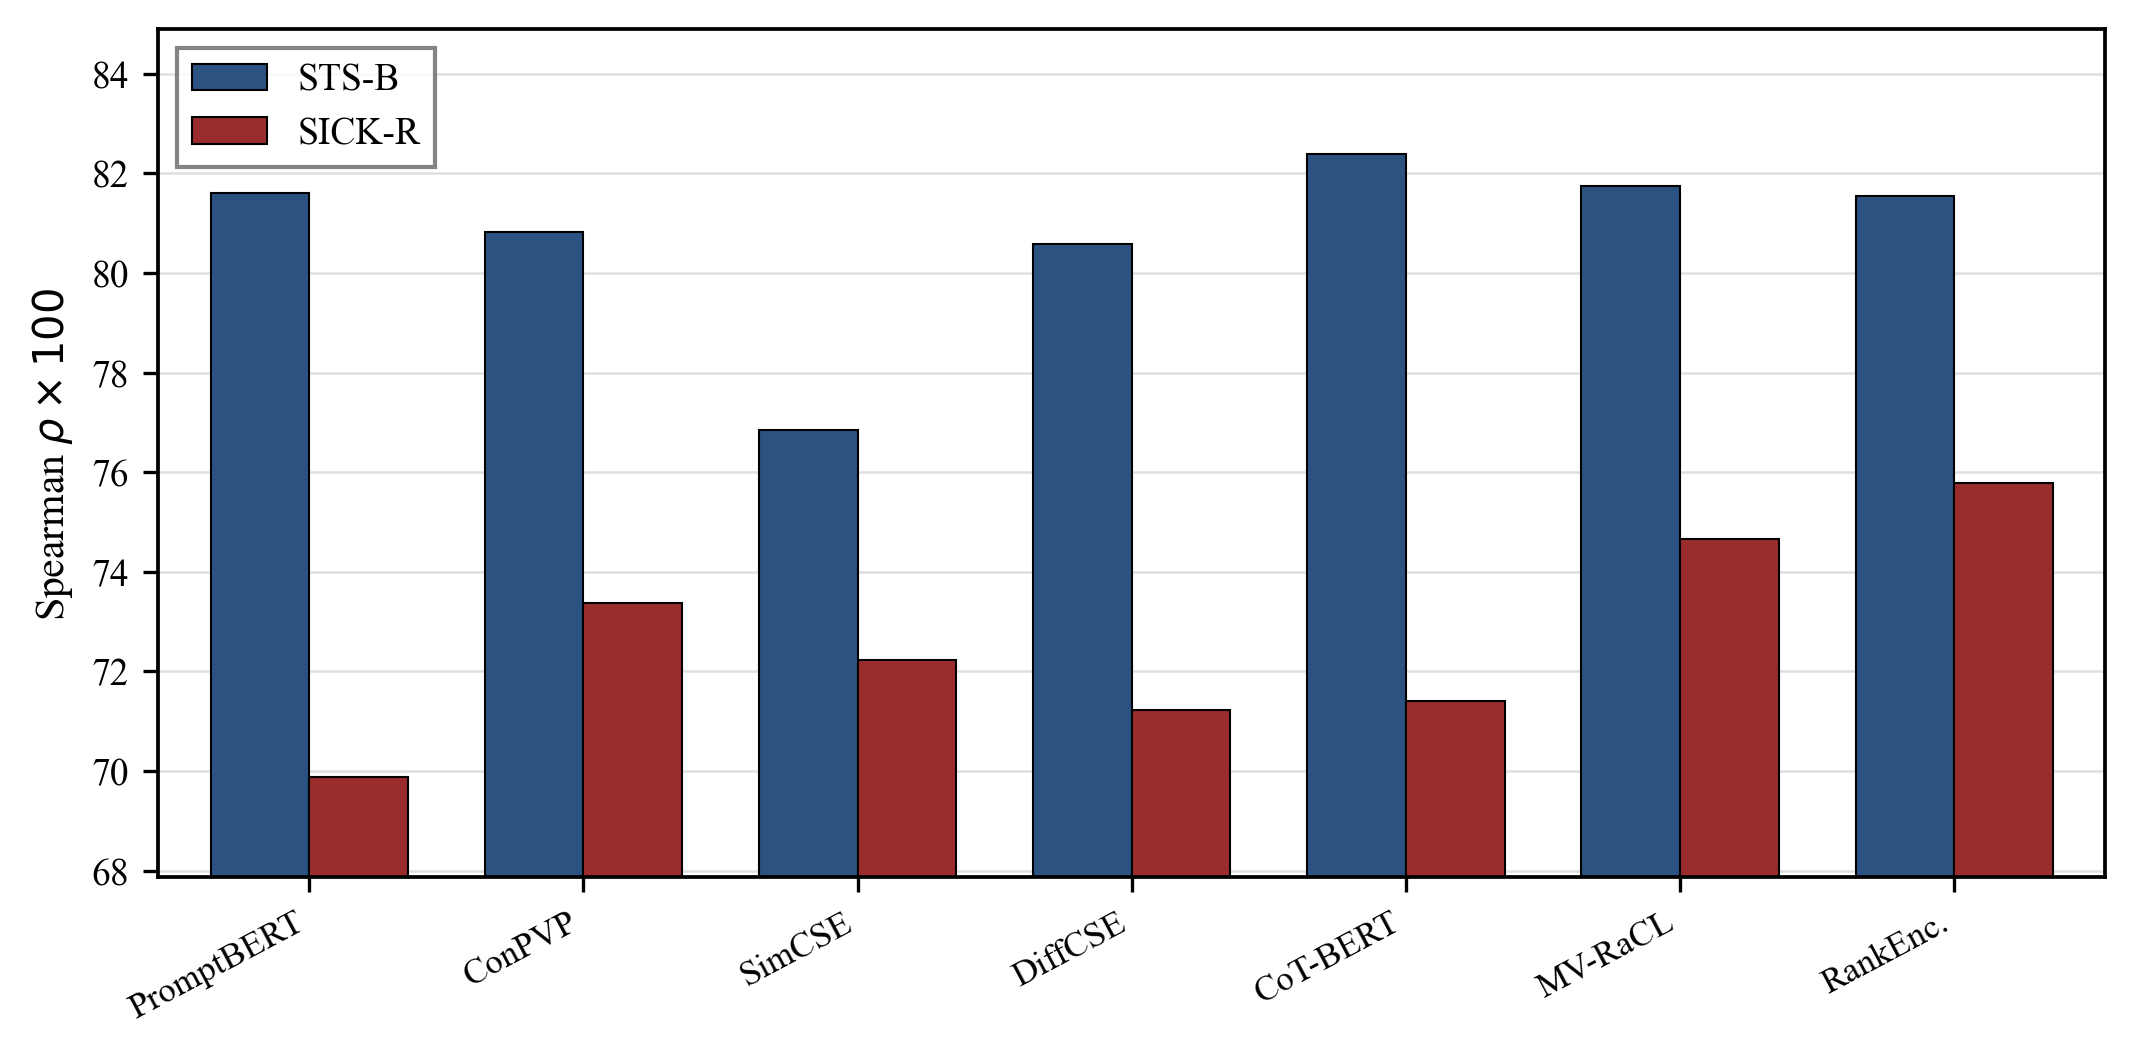
\includegraphics[width=.85\textwidth]{sts_stickr_grouped}
\caption{Comparison of STS-Benchmark and SICK-R Spearman correlations ($\rho \times 100$) for Block~1 methods in Table~\ref{tab:main}. STS-B scores do not rank methods identically to SICK-R.}
\label{fig:sts-sick}
\end{figure*}

In both the main experiments and the ablation study, we observe that the trends on the general STS suite and on SICK-R are not strictly monotone aligned (cross-metric asynchrony). Taking our method against CoT-BERT in Table~\ref{tab:main} as an example, SICK-R improves from $71.41$ to $74.65$, while STS-B drops slightly from $82.40$ to $81.75$. Such differences should not be attributed to mere implementation noise; rather, they should be understood through the interaction between evaluation-target heterogeneity and model inductive bias. Fig.~\ref{fig:sts-sick} visualizes STS-Benchmark \emph{vs.}\ SICK-R $\rho{\times}100$ for Block~1 methods in Table~\ref{tab:main}, illustrating that STS-B rankings do not coincide with those on SICK-R.

From the perspective of data construction, the linguistic phenomena measured by the STS subsets differ (cf.\ Section~\ref{subsec:setup-exp}): STS12 and STS13 emphasize lexical and topical proximity in domains such as news; STS15 stresses paraphrastic equivalence; while SICK-R systematically incorporates compositional phenomena such as negation, quantification, and relational structure~\cite{sick}, and its relatedness-score distribution is also not fully aligned with that of the STS series. Consequently, it is not a logical necessity for a single training objective to attain a monotone optimum on both benchmarks simultaneously.

From the perspective of model mechanism, the multi-view role modeling, the negation-style template, and the dual-temperature contrastive objective adopted in this work impose a stronger inductive bias on decision boundaries that require explicit discrimination of semantic opposition and fine-grained differences. As a result, gains are more pronounced under the relatedness structure emphasized by SICK-R; this does not, however, entail monotone optimality on every STS subtask under comparable model capacity. Training stochasticity, hyperparameter sensitivity, and the various ablation paths in Table~\ref{tab:ablation} can also disturb cross-metric performance, so we refrain from drawing single-factor causal conclusions about the cross-metric phenomenon.

\subsubsection{Comparison with Ranking-Augmented Methods}

Among the ranking-augmented methods in Block~2 of Table~\ref{tab:main}, RankEncoder maintains an external reference corpus and performs rank-correlation alignment. By contrast, MV-RaCL avoids external teachers and external corpora, completing end-to-end training within a single BERT-base encoder via VRIB and a dual-temperature hard-negative objective.

On SICK-R, our method ($74.65$) is substantially higher than CoT-BERT ($71.41$) and approaches RankEncoder ($75.78$). The take-away is that the relevant comparison is not point-wise optimum on a single metric, but whether external ranking dependence is introduced: ranking-augmented methods trade higher system complexity and additional resources for a better general-STS average and a higher SICK-R upper bound, whereas our method offers an end-to-end training path that requires no external teacher and no external corpus, while still delivering substantial gains on fine-grained compositional semantics relative to the direct baseline. The two families are therefore best understood as different technical routes under different resource budgets, rather than as strict substitutes under identical conditions.

%% ================================================================
%% 5. Conclusion
%% ================================================================
\section{Conclusion}
\label{sec:conclusion}

This paper presents MV-RaCL, a multi-view role-aware contrastive learning framework tailored for composition-sensitive semantic matching. Our method effectively overcomes the \emph{role-agnostic} bottleneck implicit in existing prompt-based sentence encoders by introducing a unified View-Role Inductive Bias (VRIB). We thoroughly validate MV-RaCL's superiority, demonstrating that differentiating anchor, positive, and hard-negative views across the template, encoding, and optimization levels significantly sharpens the model's compositional discrimination while preserving its general matching capabilities. Additionally, we provide an in-depth four-stage analysis---spanning representation-space geometry to pair-level tracking---to elucidate the underlying mechanisms that drive MV-RaCL's success. Future work will explore adapting this role-aware mechanism to larger generative language models and multilingual contexts.

%% ================================================================
%% References
%% ================================================================

\begin{thebibliography}{99}

\bibitem{sts3kcl}
J. Fodor, S. De Deyne, S. Suzuki, Compositionality and sentence meaning: comparing semantic parsing and transformers on a challenging sentence similarity dataset, Comput. Linguist. 51 (1) (2025) 139--190.

\bibitem{simcse}
T. Gao, X. Yao, D. Chen, SimCSE: Simple contrastive learning of sentence embeddings, in: Proceedings of the 2021 Conference on Empirical Methods in Natural Language Processing, Punta Cana, Dominican Republic, 2021, pp. 6894--6910.

\bibitem{bert}
J. Devlin, M.-W. Chang, K. Lee, K. Toutanova, BERT: Pre-training of deep bidirectional transformers for language understanding, in: Proceedings of the 2019 Conference on the North American Chapter of the Association for Computational Linguistics: Human Language Technologies, Volume 1 (Long and Short Papers), Minneapolis, MN, USA, 2019, pp. 4171--4186.

\bibitem{promptbert}
T. Jiang, J. Jiao, S. Huang, Z. Zhang, D. Wang, F. Zhuang, F. Wei, H. Huang, D. Deng, Q. Zhang, PromptBERT: Improving BERT sentence embeddings with prompts, in: Proceedings of the 2022 Conference on Empirical Methods in Natural Language Processing, Abu Dhabi, UAE, 2022, pp. 8826--8837.

\bibitem{cotbert}
B. Zhang, K. Chang, C. Li, CoT-BERT: Enhancing unsupervised sentence representation through chain-of-thought, in: International Conference on Artificial Neural Networks (ICANN), Lecture Notes in Computer Science, Springer Nature, Cham, Switzerland, 2024.

\bibitem{sick}
M. Marelli, S. Menini, M. Baroni, L. Bentivogli, R. Bernardi, R. Zamparelli, A SICK cure for the evaluation of compositional distributional semantic models, in: Proceedings of the Ninth International Conference on Language Resources and Evaluation (LREC 2014), Reykjavik, Iceland, 2014.

\bibitem{rankcse}
J. Liu, J. Liu, Q. Wang, Y. Wang, W. Cai, D. Sheng, R. Xu, J. Yu, RankCSE: Unsupervised sentence representations learning via learning to rank, in: Proceedings of the 61st Annual Meeting of the Association for Computational Linguistics (Volume 1: Long Papers), Toronto, Canada, 2023.

\bibitem{rankencoder}
Y. Lee, S. Hong, S. Park, J. Kim, J. Park, S. Hwang, Ranking-enhanced unsupervised sentence representation learning, in: Proceedings of the 61st Annual Meeting of the Association for Computational Linguistics (Volume 1: Long Papers), Toronto, Canada, 2023.

\bibitem{raoe}
Z. Zhou, M. Huang, Q. Miao, Rank-awareness and angular constraints: a new perspective on learning sentence embeddings from NLI data, in: Proceedings of the 2025 Conference on Empirical Methods in Natural Language Processing (EMNLP 2025), Suzhou, China, 2025.

\bibitem{nguyen2026embedtrace}
M.A. Nguyen, K. Sai, M. Nguyen, Tracing the evolution of word embedding techniques in natural language processing, 2026, arXiv preprint arXiv:2603.13271.

\bibitem{kurz2026tacl}
S. Kurz, J.-J. Chen, L. Flek, Z. Zhao, On the limitations of language-targeted pruning: investigating the calibration language impact in multilingual LLM pruning, Trans. Assoc. Comput. Linguist. 14 (2026) 167--192.

\bibitem{isbert}
Y. Zhang, R. He, Z. Liu, K.H. Lim, L. Bing, An unsupervised sentence embedding method by mutual information maximization, in: Proceedings of the 2020 Conference on Empirical Methods in Natural Language Processing (EMNLP), Online, 2020, pp. 1601--1610.

\bibitem{consert}
Y. Yan, R. Li, S. Wang, F. Zhang, W. Wu, W. Xu, ConSERT: A contrastive framework for self-supervised sentence representation transfer, in: Proceedings of the 59th Annual Meeting of the Association for Computational Linguistics (Volume 1), Virtual, 2021, pp. 7945--7959.

\bibitem{alignment}
T. Wang, P. Isola, Understanding contrastive representation learning through alignment and uniformity on the hypersphere, in: Proceedings of the 37th International Conference on Machine Learning (ICML), Virtual Conference, USA, 2020, pp. 8927--8936.

\bibitem{diffcse}
Y.S. Chuang, et al., DiffCSE: Difference-based contrastive learning for sentence embeddings, in: Proceedings of the 2022 Conference of the North American Chapter of the Association for Computational Linguistics: Human Language Technologies, Seattle, WA, USA, 2022.

\bibitem{esimcse}
X. Wu, C. Gao, L. Zang, J. Han, Z. Wang, S. Hu, ESimCSE: Enhanced sample building method for contrastive learning of unsupervised sentence embedding, in: Proceedings of the 29th International Conference on Computational Linguistics (COLING), Gyeongju, Republic of Korea, 2022.

\bibitem{pcl}
Q. Wu, C. Tao, T. Shen, C. Xu, X. Geng, D. Jiang, PCL: Peer-contrastive learning with diverse augmentations for unsupervised sentence embeddings, in: Proceedings of the 2022 Conference on Empirical Methods in Natural Language Processing (EMNLP), Abu Dhabi, UAE, 2022.

\bibitem{arccse}
Y. Zhang, H. Zhu, Y. Wang, N. Xu, X. Li, B. Zhao, A contrastive framework for learning sentence representations from pairwise and triple-wise perspective in angular space, in: Proceedings of the 60th Annual Meeting of the Association for Computational Linguistics (Volume 1), Dublin, Ireland, 2022.

\bibitem{angle}
X. Li, J. Li, AoE: Angle-optimized embeddings for semantic textual similarity, in: Proceedings of the 62nd Annual Meeting of the Association for Computational Linguistics (Volume 2), Bangkok, Thailand, 2024.

\bibitem{sncse}
H. Wang, et al., SNCSE: Contrastive learning for unsupervised sentence embedding with soft negative samples, 2022, arXiv preprint arXiv:2201.05979.

\bibitem{e5}
L. Wang, et al., Text embeddings by weakly-supervised contrastive pre-training, 2022, arXiv preprint arXiv:2212.03533.

\bibitem{gte}
X. Zhang, et al., mGTE: Generalized long-context text representation and reranking models for multilingual text retrieval, in: Proceedings of the 2024 Conference on Empirical Methods in Natural Language Processing (EMNLP), Miami, FL, USA, 2024.

\bibitem{promcse}
Y. Jiang, L. Zhang, W. Wang, Improved universal sentence embeddings with prompt-based contrastive learning and energy-based learning, in: Findings of the Association for Computational Linguistics: EMNLP 2022, Abu Dhabi, UAE, 2022.

\bibitem{conpvp}
J. Zeng, Y. Yin, Y. Jiang, S. Wu, Y. Cao, Contrastive learning with prompt-derived virtual semantic prototypes for unsupervised sentence embedding, in: Findings of the Association for Computational Linguistics: EMNLP 2022, Abu Dhabi, UAE, 2022, pp. 7042--7053.

\bibitem{senteval}
A. Conneau, D. Kiela, SentEval: An evaluation toolkit for universal sentence representations, in: Proceedings of the Eleventh International Conference on Language Resources and Evaluation (LREC 2018), Miyazaki, Japan, 2018.

\bibitem{dclr}
K. Zhou, B. Zhang, X. Zhao, J.R. Wen, Debiased contrastive learning of unsupervised sentence representations, in: Proceedings of the 60th Annual Meeting of the Association for Computational Linguistics (Volume 1), Dublin, Ireland, 2022, pp. 6120--6130.

\bibitem{sunctxsim}
X. Sun, Y. Meng, X. Ao, F. Wu, T. Zhang, J. Li, C. Fan, Sentence similarity based on contexts, Trans. Assoc. Comput. Linguist. 10 (2022) 573--588.

\bibitem{sbert}
N. Reimers, I. Gurevych, Sentence-BERT: Sentence embeddings using Siamese BERT-networks, in: Proceedings of the 2019 Conference on Empirical Methods in Natural Language Processing (EMNLP), Hong Kong, China, 2019, pp. 3983--3992.

\bibitem{mexma}
J.M. Janeiro, B. Piwowarski, P. Gallinari, L. Barrault, MEXMA: Token-level objectives improve sentence representations, in: Proceedings of the 63rd Annual Meeting of the Association for Computational Linguistics (ACL), Vienna, Austria, 2025.

\bibitem{sct}
P. Limkonchotiwat, et al., An efficient self-supervised cross-view training for sentence embedding, Trans. Assoc. Comput. Linguist. 11 (2023) 1572--1587.

\bibitem{unsee}
O. Cagatan, UNSEE: Unsupervised non-contrastive sentence embeddings, in: Proceedings of the 18th Conference of the European Chapter of the Association for Computational Linguistics (EACL), St. Julian's, Malta, 2024.

\bibitem{tempcooldown}
Y.H. Jeong, M.S. Han, D.K. Chae, Simple temperature cool-down in contrastive framework for unsupervised sentence representation learning, in: Findings of the Association for Computational Linguistics (EACL 2024), St. Julian's, Malta, 2024.

\bibitem{kdmcse}
C.D. Nguyen, T. Nguyen, X. Wu, A.T. Luu, KDMCSE: Knowledge distillation multimodal sentence embeddings with adaptive angular margin contrastive learning, in: Proceedings of the 2024 Conference of the North American Chapter of the Association for Computational Linguistics (NAACL), Mexico City, Mexico, 2024.

\bibitem{anglebased}
Y.H. Jeong, M. Han, D.K. Chae, A simple angle-based approach for contrastive learning of unsupervised sentence representation, in: Findings of the Association for Computational Linguistics: EMNLP 2024, Miami, FL, USA, 2024.

\bibitem{threer}
L. Ma, X. Wu, Y. Huang, S. Gao, Z. Yu, 3R: Enhancing sentence representation learning via redundant representation reduction, in: Proceedings of the 2025 Conference on Empirical Methods in Natural Language Processing (EMNLP 2025), Suzhou, China, 2025.

\bibitem{mteb}
N. Muennighoff, N. Tazi, L. Magne, N. Reimers, MTEB: Massive text embedding benchmark, in: Proceedings of the 17th Conference of the European Chapter of the Association for Computational Linguistics (EACL), Dubrovnik, Croatia, 2023.

\bibitem{hypercl}
Y. Yoo, J. Cha, C. Kim, T. Kim, Hyper-CL: Conditioning sentence representations with hypernetworks, in: Proceedings of the 62nd Annual Meeting of the Association for Computational Linguistics (ACL), Bangkok, Thailand, 2024.

\end{thebibliography}


\vspace{-15mm}

\begin{IEEEbiography}[{
\includegraphics[width=0.8in,height=1in,clip,keepaspectratio]{luminfeng.jpg}}]{Minfeng Lu}
received the M.S.\ degree in computer science and technology from Zhejiang University, Hangzhou, China.
He is currently an Assistant Professor with the Department of Modern Information Technology at Zhejiang Polytechnic University of Mechanical and Electrical Engineering, Hangzhou.
His research interests include machine learning, deep learning, and natural language processing (NLP).
\end{IEEEbiography}

\vspace{-15mm}

\begin{IEEEbiography}[{
\includegraphics[width=0.8in,height=1in,clip,keepaspectratio]{zhangqifei.png}}]{Qifei Zhang}
received the Ph.D.\ degree in computer science and technology from Zhejiang University, Hangzhou, China.
He is currently an Associate Professor with the Department of Software Technology at Zhejiang University.
His research interests include operating systems, industrial internet, trusted computing, and machine learning.
\end{IEEEbiography}

\vspace{-15mm}

\begin{IEEEbiography}[{
\includegraphics[width=0.8in,height=1in,clip,keepaspectratio]{qinhanlin.png}}]{Hanlin Qin}
is currently a Lecturer with the School of Artificial Intelligence at Zhejiang Polytechnic University of Mechanical and Electrical Engineering, Hangzhou, China.
His research focuses on machine learning and deep learning, especially representation learning and model design for perceptual tasks such as computer vision.
\end{IEEEbiography}

\vspace{-15mm}

\begin{IEEEbiography}[{
\includegraphics[width=0.8in,height=1in,clip,keepaspectratio]{zouhuilai.png}}]{Huilai Zou}
received the M.S.\ degree in computer science from Zhejiang Normal University, Jinhua, China.
He is currently an Associate Professor with the Department of Modern Information Technology at Zhejiang Polytechnic University of Mechanical and Electrical Engineering, Hangzhou.
His research interests include software engineering, artificial intelligence, and machine learning.
\end{IEEEbiography}

\end{document}
